% !TeX spellcheck = en_US
\documentclass[english,master,dept460,male,cpp,cpdeclaration]{diploma}
\setcounter{tocdepth}{3}

% pdflatex.exe -synctex=1 -interaction=nonstopmode --shell-escape --aux-directory=./Auxiliary %.tex
% biber.exe --output_directory Auxiliary %

\RequirePackage[autostyle = true]{csquotes}
\RequirePackage[backend = biber, style = numeric, alldates = iso, seconds = true, sorting = none]{biblatex}
\RequirePackage[bottom, multiple]{footmisc}
\RequirePackage{dcolumn}
\RequirePackage{subfig}
\RequirePackage{enumitem}
\RequirePackage{float}
\RequirePackage{tabularx}
\RequirePackage{multirow}
\RequirePackage{amsmath}
\RequirePackage{xfrac}
\RequirePackage{tikz}
\RequirePackage{pgfplots}
\RequirePackage{adjustbox}
\RequirePackage{diagbox}
\RequirePackage{varwidth}
\RequirePackage{letltxmacro}

% CONDITIONAL SETUP

\newbool{VSB}
%\booltrue{VSB}
\boolfalse{VSB}

% COMMAND SETUP

\newcolumntype{d}[1]{D{.}{.}{#1}}
\newcolumntype{f}[1]{>{\centering\let\newline\\\arraybackslash\hspace{0pt}}p{#1}}

\setlist{
	beginpenalty = 10000,
	listparindent = \parindent,
	parsep = 0pt
}

\makeatletter
\renewcommand\paragraph
	{\@startsection{paragraph}{4}{\z@}
	{-3.25ex plus 1ex minus .2ex}
	{1.5ex plus .2ex}
	{\normalfont\normalsize\bfseries}}
\renewcommand\subparagraph
	{\@startsection{subparagraph}{5}{\z@}
	{-3.25ex plus 1ex minus .2ex}
	{1.5ex plus .2ex}
	{\normalfont\normalsize\bfseries}}

\global\let\TX@vwarn\@empty % disable \verb in tabularx warning
\makeatother

\newcommand{\subfoursection}[1]{\paragraph{#1}}
\newcommand{\subfivesection}[1]{\subparagraph{#1}}
\newcommand{\nosep}{\itemsep0em}
\newcommand{\pair}[2]{$\,\langle\,#1,\,#2\,\rangle$}
\newcommand{\triple}[3]{$\,\langle\,#1,\,#2,\,#3\,\rangle$}

\let\thorn\th
\renewcommand{\th}[1]{\hspace*{\fill}{#1}\hspace*{\fill}}
\newcommand{\fixcline}{\\[-\arrayrulewidth]}

\newcommand{\tikzfigure}[1]{
	\tikzsetnextfilename{#1}%
	\input{Figures/TikZ/#1.tex}%
}

\newcommand{\texfigure}[1]{
	\input{Figures/TeX/#1}%
}

\usetikzlibrary{external, fit, positioning, patterns}
\tikzexternalize[prefix = Generated/]

\usepgfplotslibrary{statistics}
\pgfplotsset{compat = 1.16}
\pgfplotsset{cycle list name = exotic}
\pgfkeys{/pgf/number format/.cd,1000 sep={\,}}

% THESIS METADATA

\ThesisAuthor{Daniel Chýlek}
\SubmissionDate{April 30, 2020}

\EnglishThesisTitle{Brotli Compression Algorithm}

\EnglishAbstract{This thesis is a comprehensive exploration of the Brotli compression algorithm and data format. After explaining key principles Brotli is built upon, the paper introduces a custom implementation that provides tools to study the format and develop new format-compatible compression techniques. The custom implementation is followed by an in-depth look at the official compressor implementation, and how different quality levels utilize features of the format. The paper concludes by using the gained insight to experiment with the format and compression techniques.}

\EnglishKeywords{lossless compression; Brotli; Huffman coding; context modeling}

\ifbool{VSB}{
	
\CzechThesisTitle{Kompresní metoda Brotli}

\CzechAbstract{Tato práce je obsáhlým průzkumem kompresní metody Brotli a souvisejícího formátu dat. Úvodní vysvětlení klíčových principů Brotli je následováno představením vlastní implementace, jejíž cílem je zjednodušit studování formátu a vývoje nových metod komprese kompatibilních s formátem Brotli. Další část práce podrobně zkoumá oficiální implementaci kompresoru, a to jak různé kompresní úrovně využívají možnosti formátu, včetně detailního popisu jejich implementace. Práce je zakončena experimentálními úpravami oficiálního kompresoru s cílem zlepšení komprese bez narušení kompatibility formátu dat.}

\CzechKeywords{bezztrátová komprese; Brotli; Huffmanovo kódování; kontextové modelování}

\ThesisAssignmentImagePath{Figures/Assignment}
\AuthorDeclarationImageFile{Figures/Declaration}

}{

\Thanks{

\noindent
\textbf{Foreword}
\medbreak
\noindent
You are reading an online version of my masters thesis. The source codes and issue tracker are available at \url{https://github.com/chylex/Brotli-Builder}.
\medbreak
\noindent
I would like to thank doc. Ing. Jan Platoš, Ph.D. for leading and supervising the project.

\vspace{50pt}

\noindent
\textbf{Updates}
\medbreak
\noindent
\begin{tabular}{@{}lcl}
	24 July 2020 & & Corrected minor visual issue with GUI application image. \\
\end{tabular} 

\vspace{50pt}
}}

\setboolean{Dipl@PrintCooperatingPersonsDeclaration}{false}

\AddAcronym{API}{Application Programming Interface}
\AddAcronym{CLI}{Command Line Interface}
\AddAcronym{CRLF}{Carriage Return \texttt{+} Line Feed}
\AddAcronym{CSS}{Cascading Style Sheets}
\AddAcronym{GUI}{Graphical User Interface}
\AddAcronym{HTML}{Hypertext Markup Language}
\AddAcronym{HTTP}{Hypertext Transfer Protocol}
\AddAcronym{JS}{JavaScript}
\AddAcronym{LZ77}{Lempel-Ziv 77}
\AddAcronym{MSVC}{Microsoft Visual C++}
\AddAcronym{RFC}{Request for Comments}
\AddAcronym{SDK}{Software Development Kit}
\AddAcronym{UTF}{Unicode Transformation Format}
\AddAcronym{\texttt{\textvisiblespace}}{Indicates a single space character}
\AddAcronym{\texttt{B}}{Byte (8 bits)}
\AddAcronym{\texttt{KiB}}{Kibibyte, \texttt{1 KiB} = \texttt{1024 B}}
\AddAcronym{\texttt{MiB}}{Mebibyte, \texttt{1 MiB} = \texttt{1024 KiB}}
\AddAcronym{\texttt{GiB}}{Gibibyte, \texttt{1 GiB} = \texttt{1024 MiB}}

\addbibresource{References/sources.bib}

\begin{document}
\MakeTitlePages

% SOURCE CODE THEME

\definecolor{lstdefault}{HTML}{171717}
\definecolor{lstkeywords}{HTML}{0101FD}
\definecolor{lstcomments}{HTML}{008000}
\definecolor{lststrings}{HTML}{A31515}
\definecolor{lsttypes}{HTML}{007D9A}

\lstset{
	language = [Sharp]C,
	columns = fixed,
	basewidth = 0.5em,
	inputencoding = utf8,
	extendedchars = true,
	literate =
		{␣}{{\textvisiblespace}}1
		{𝟎}{{{\color{lststrings}0}}}1
		{𝟏}{{{\color{lststrings}1}}}1
		{𝟐}{{{\color{lststrings}2}}}1
		{𝟑}{{{\color{lststrings}3}}}1
		{𝟒}{{{\color{lststrings}4}}}1
		{𝟓}{{{\color{lststrings}5}}}1
		{𝟔}{{{\color{lststrings}6}}}1
		{𝟕}{{{\color{lststrings}7}}}1
		{𝟖}{{{\color{lststrings}8}}}1
		{𝟗}{{{\color{lststrings}9}}}1,
	emph = {
		BrotliGlobalState,
		BrotliFileParameters,
		BrotliCompressionParameters,
		CompressedMetaBlockBuilder,
		ContextMapBuilder,
		Literals,
		Distances,
		Category,
		Literal,
		IntRange
	},
	morekeywords = {
		var
	},
	identifierstyle = \color{lstdefault},
	commentstyle = \color{lstcomments},
	keywordstyle = \color{lstkeywords},
	stringstyle = \color{lststrings},
	emphstyle = \color{lsttypes}
}

% THESIS CONTENTS

\section{Introduction}

Brotli is a general-purpose lossless compression algorithm developed by Google, Inc. It defines a bit-oriented format inspired by DEFLATE\cite{RFC1951}, which is in essence a combination of LZ77 and Huffman coding. Brotli aims to replace DEFLATE in HTTP compression by providing better compression ratios and more flexibility than current standards.

This thesis introduces a program library, which implements Brotli compression and decompression based on the RFC7932\cite{RFC7932} specification, as well as several utility applications intended to aid understanding and analysis of Brotli compressed files. This is followed by an in-depth exploration of the official implementation, and the differences between it and the custom implementation. The insight gained by studying the format is used to propose and test several experimental modifications to the official implementation, which intend to improve compression while maintaining format compatibility.

Section \ref{sec:setup-and-organization} describes the organization of the programming projects, information about the software setup, and the compression corpus used for testing and validation. The section ends with a comparison between Brotli, and both current and upcoming HTTP compression standards.

Section \ref{sec:explaining-brotli} explains important compression techniques, and details their use in the Brotli format. It also introduces Brotli-specific concepts and terminology.

Section \ref{sec:implementing-brotli} talks about the technical background of the main program library, decisions that went into the custom implementation, and examples of how the library API can be used.

Section \ref{sec:official-implementation} explores the official compressor implementation and advanced features of the format. The first part points out differences between quality levels. The second part describes and evaluates official implementations of individual features. The third part concludes with several experiments that modify the official source code in an attempt to find improvements.

\section{Setup \& Organization}
\label{sec:setup-and-organization}
	
	\subsection{Project Organization}
	
	The custom implementation and utilities were written in \verb|C# 8|, and organized into several projects in a Visual Studio 2019 solution:
	
	\bigskip
	\noindent
	\begin{tabularx}{\textwidth}{ l | l | l | X }
	Name & Type & Framework & Description \\
	\hline
	\verb|Brotli|\hspace{2.5pt}\verb|Lib| & Library & \verb|.NET Standard 2.1| & Main library --- implementation of Brotli \\
	\verb|Brotli|\hspace{2.5pt}\verb|Impl| & Library & \verb|.NET Standard 2.1| & Example uses of the main library API \\
	\verb|Brotli|\hspace{2.5pt}\verb|Builder| & GUI\footnote{The GUI is based on Windows Forms, which requires \verb|Desktop Runtime| to be installed alongside \verb|.NET Core|.} & \verb|.NET Core 3.0| & Utility for file analysis \& comparison \\
	\verb|Brotli|\hspace{2.5pt}\verb|Calc| & CLI & \verb|.NET Core 3.0| & Utility for batch file processing \\
	\end{tabularx}
	
	\bigskip
	\noindent
	\ifbool{VSB}{
		All projects are included in the attachment.
	}{
		All projects are available at \url{https://github.com/chylex/Brotli-Builder}.
	}
	
	\subsection{Brotli Compilation}
	\label{sec:brotli-compilation}
	
	The Brotli executable and all its modified versions were built using the official repository at \url{https://github.com/google/brotli}, and based on the \verb|c435f06| commit from October 1, 2019. This version included a few improvements committed after the official v1.0.7 release. The following software configuration was used for all builds:
	
	\begin{itemize} \nosep
		\item \verb|Visual Studio 2019 (16.3.9)|
		\item \verb|LLVM 8.0.1|
		\item \verb|MSVC 14.23.28105|
		\item \verb|Windows SDK 10.0.18362.0|
		\item \verb|clang_cl_x64| toolset
		\item \verb|Release| configuration
	\end{itemize}
	
	\subsection{Test Data}
	
	Brotli was designed with multilingual text and web languages encoded with the UTF-8 standard in mind, but it is still able to reasonably compress text in other encoding systems, and certain kinds of binary data.
	
	A mixed corpus was built for testing and analysis of both the custom implementation, and individual features of the official compressor.
	
	The corpus includes commonly used lossless compression corpora, which have a variety of text and binary formats, as well as a collection of multilingual texts and website resources. Files gathered outside of existing corpora were selected to represent the kind of data Brotli is intended for, and thus should benefit from its features and heuristics.
	
	The corpus includes 169 files totaling $\approx$ \verb|263 MiB| (median $\approx$ \verb|54.5 KiB|). \ifbool{VSB}{All files were made available in the attachment.}{All files were made available at \url{https://github.com/chylex/Brotli-Builder/blob/master/Paper/Corpus.7z}.}
	
	\begin{itemize} \nosep
		\item The Canterbury Corpus\footnote{\url{http://corpus.canterbury.ac.nz/descriptions/\#cantrbry}} (\verb|2.7 MiB|)
		\item The Silesia Corpus\footnote{\url{http://sun.aei.polsl.pl/~sdeor/index.php?page=silesia}} (\verb|202 MiB|)
		\item A selection of files from Snappy Test Data\footnote{\url{https://github.com/google/snappy/tree/e9e11b84e629c3e06fbaa4f0a86de02ceb9d6992/testdata}} (\verb|1.7 MiB|)
		\begin{itemize} \nosep
			\item fireworks.jpeg, geo.protodata, html, html\_x\_4, kppkn.gtb, paper-100k.pdf, urls.10K
		\end{itemize}
		\item The Bible in various languages (\verb|37 MiB|)
		\begin{itemize} \nosep
			\item Arabic\footnote{\url{https://ebible.org/find/details.php?id=arbnav}},
			      Chinese (Simplified)\footnote{\url{https://ebible.org/find/details.php?id=cmn-cu89s}},
			      Chinese (Traditional)\footnote{\url{https://ebible.org/find/details.php?id=cmn-cu89t}},
			      English\footnote{\url{https://ebible.org/find/details.php?id=eng-asv}},
			      Hindi\footnote{\url{https://ebible.org/find/details.php?id=hin2017}},
			      Russian\footnote{\url{https://ebible.org/find/details.php?id=russyn}},
			      Spanish\footnote{\url{https://ebible.org/find/details.php?id=spaRV1909}}
			\item Each language was downloaded in the \emph{Plain text canon only chapter files} format. Text files from each archive were combined with a new line (\verb|CRLF|) following each file.
		\end{itemize}
		\item \verb|HTML|, \verb|CSS|, and \verb|JS| files from several of the most popular websites (\verb|20.4 MiB|)
		\begin{itemize} \nosep
			\item \url{baidu.com}, \url{facebook.com}, \url{google.com}, \url{instagram.com}, \url{vk.com}, \url{wikipedia.org}, \url{yandex.ru}, \url{youtube.com}
			\item Each website was downloaded using the \emph{Save page as...}, \emph{Web Page, complete} feature in an anonymous window in Firefox.
		\end{itemize}
	\end{itemize}
	
		\subsubsection{Brotli vs. gzip vs. zstd}
		
		As Brotli targets HTTP compression, it makes sense to compare it to \verb|gzip|, the currently most used HTTP compression method, and \verb|zstd|, a new compression standard developed by Facebook.
		
		This comparison only considers out-of-the-box results for each quality level. Although both Brotli and \texttt{zstd} include options for using large amounts of memory to improve compression, their use would not be reasonable for websites. Additionally, with support for custom dictionaries in \verb|zstd| and upcoming support in Brotli, website owners could put additional effort into optimization.
		
		While this is only a total size comparison, for HTTP compression it is also important to consider compression speeds at each quality level. The highest quality levels may not be suitable for on-the-fly compression, but could be used to pre-compress and serve static content.
		
		Figure \ref{fig:test-corpus-comparison} shows the size comparison between Brotli, \verb|gzip 1.10|, and \verb|zstd 1.4.4|.
		
		\begin{figure}[H]
			\tikzfigure{test-corpus-comparison}
			\caption{Test corpus size comparison between Brotli, gzip, and zstd.}
			\label{fig:test-corpus-comparison}
		\end{figure}

\section{Explaining Brotli}
\label{sec:explaining-brotli}

A Brotli compressed file or data stream comprises a \emph{stream header} and a sequence of \emph{meta-blocks}. A meta-block may be empty --- optionally skipping part of the data stream --- or it can contain output bytes in either uncompressed or compressed form. In the interest of brevity, assume that any mentions of meta-blocks, which do not explicitly specify their type, concern compressed meta-blocks.

Each meta-block begins with a header describing its type, size of uncompressed output (with an upper limit of \verb|16 MiB|), and other type-dependent metadata. The header is immediately followed by a data section. In compressed meta-blocks, the data section is a sequence of commands, and the header includes all information needed to decode these commands.

To understand Brotli, we will look at the pieces that form a compressed meta-block, and how they fit together to generate uncompressed output bytes. The next few sections briefly introduce important concepts, many of which are also found in other kinds of compression algorithms and thus are not unique to Brotli.

	\subsection{Huffman Coding}
	
	Binary Huffman coding encodes \emph{symbols} of an \emph{alphabet} using variable-length bit sequences\cite{Huffman}. The intention is that we can take a sequence of symbols, and construct a code that represents frequent symbols with short bit sequences, and infrequent symbols with long bit sequences. This by itself is a form of compression, and can be used to compress files by treating individual byte values as symbols.
	
	Brotli makes heavy use of Huffman coding to encode not only individual bytes of the uncompressed output, but also various special codes that command the process of decompression.
	
	We will define a Huffman tree as a full binary tree, where each leaf represents one symbol. Given a sequence of input bits, we start traversing the tree from its root, go down the left branch whenever we encounter a $0$, go down the right branch whenever we encounter a $1$, and output a symbol after reaching a leaf node. If any input bits remain, the traversal restarts at the root.
	
	An example of such tree with a 3-symbol alphabet $\{a, b, c\}$ is shown in figure \ref{fig:huffman-tree}. In this example, the bit sequence $001011$ would unambiguously map to the symbol sequence $aabc$.
	
	\begin{figure}[H]
		\centering
		\medskip
		
		\noindent
		\begin{minipage}{0.22\textwidth}
			\centering
			\tikzfigure{huffman-tree-example}
		\end{minipage}%
		\begin{minipage}{0.22\textwidth}
			\centering
			
			\begin{tabular}{c|l}
				a & 0 \\
				\hline
				b & 10 \\
				\hline
				c & 11 \\
			\end{tabular}
			
		\end{minipage}
	
		\caption{Huffman tree containing paths to 3 symbols.}
		\label{fig:huffman-tree}
	\end{figure}
	
	\subsection{Intermediary Codes}
	
	Oftentimes, we want to encode a potentially very large range of values, with the assumption that small values are more likely to appear than large values.
	
	Based on this assumption, Brotli defines several sets of codes used in various parts of the format. We will call them \emph{intermediary codes}.
	
	An intermediary code has a range of possible values. To obtain a concrete value within that range, we read a certain amount of \emph{extra bits} from the bit stream, and add their value to the lower bound of the range. The difference between the upper bound and lower bound is therefore always a power of two.
	
	Figure \ref{fig:intermediary-code-example} demonstrates how an example set of 4 intermediary codes could be used to encode values between 1 and 21. Codes and their respective lower bounds are highlighted with different colors.
	
	\begin{figure}[H]
		\centering
		\smallskip
		\texfigure{intermediary-code-example}
		\caption{Example of an intermediary code set on the left, and several bit sequences and their calculated values on the right.}
		\label{fig:intermediary-code-example}
	\end{figure}

	\subsection{Sliding Window}
	
	A sliding window is a fixed-size buffer containing the most recently generated uncompressed output, which can be referenced to repeat previously seen data. This technique is the backbone of LZ77\cite{LZ77}, which has in turn influenced DEFLATE and eventually Brotli.
	
	The Brotli format specification allows for windows sizes ranging from approximately \verb|1 KiB| to \verb|16 MiB|, although more recent versions of Brotli unofficially extend the size limit up to \verb|1 GiB| which could be useful for large files outside HTTP compression.\footnote{\url{https://groups.google.com/forum/\#!topic/brotli/aq9f-x\_fSY4}}
	
	\subsection{Static Dictionary}
	
	A dictionary holds sequences of bytes. In dictionary-based compression, sequences of bytes are replaced with references to matching sequences in the dictionary --- for example, if the dictionary is a contiguous stream of bytes, a reference may be encoded as a \pair{position}{length} pair.
	
	A sliding window can be considered a kind of \emph{dynamic dictionary}, as its referenceable contents change with each newly output byte. In contrast, a \emph{static dictionary} is immutable during the entire process of decompression.\cite{DataCompressionCompleteReference}
	
	Although static dictionaries are inflexible and target only certain kinds of data --- a dictionary of English words should work best when compressing an English book --- if the same dictionary is used to compress multiple files, the overhead from storing it or obtaining it for the first time becomes negligible --- for example, if a website uses the same dictionary for all its resource files, it only needs to be downloaded once.
	
	Brotli defines a static dictionary with $13\,504$ \emph{words}. A word is an arbitrary sequence of bytes, however most commonly they are words or phrases from spoken languages, and strings found in markup and programming languages used on the web.\footnote{The dictionary is part of Brotli's focus on HTTP compression. According to its developers, the words were selected from a multilingual web corpus of 93 languages\cite{BrotliComparisonStudy}.} Words are grouped by their length, which ranges from 4 to 24 bytes, and a dictionary reference is made of the word's length group and its index within that group.
	
	This dictionary is part of the Brotli standard and can be used in all Brotli compressed files. Brotli intends to also support custom dictionaries as an extension of the Brotli format, however at the time of writing the new standard has not been finalized yet.
	
		\subsubsection{Word Transformations}
		\label{sec:dictionary-word-transformations}
		
		One distinct feature of the static dictionary in Brotli is its word transformation system. A~transform applies one of the available preset functions to the word itself, and may also add a prefix and/or a suffix. There are 121 different transforms applicable to all words, for a total of 1.6~million words.\footnote{While $1\,633\,984$ is the total amount of words representable by a dictionary reference, listing every possible word shows that only $1\,399\,565$ are unique.}
		
		These are the available functions:
		
		\begin{itemize} \nosep
			\item \textbf{Identity} does not change the word
			\item \textbf{Omit First 1--9} removes the first 1--9 bytes of the word
			\item \textbf{Omit Last 1--9} removes the last 1--9 bytes of the word
			\item \textbf{Ferment All} splits the word into 1--3 byte UTF-8 code points, and performs a bitwise operation\footnote{The bitwise operation has no unifying meaning in terms of alphabetical characters, but we can still observe certain patterns that exploit how UTF-8 is laid out, whether by intention or coincidence. For all 1-byte code points, the transformation converts the lower case letters a--z to upper case. For some 2-byte code points, it toggles case of certain accented and non-latin alphabet letters. Note that the function does not handle 4-byte code points at all, and instead treats them as 3-byte code points --- the 4-byte case would be triggered by 3 words in the dictionary, but those words are patterns of bytes (such as four \texttt{255} bytes followed by four \texttt{0} bytes) rather than words from languages.} on all code points
			\item \textbf{Ferment First} is similar, but it only performs the operation on the first code point
		\end{itemize}
		
		\noindent
		In a dictionary reference, the transform ID (0--120) is encoded as part of the index within its word length group. For the 4-byte word length group containing 1024 words, indices 0--1023 use transform ID 0, indices 1024--2047 use transform ID 1, and so on.
		
		To better understand the capability of the transformation system, table \ref{table:dictionary-transform-examples} shows a few concrete transforms defined in the format, each with an example word transformation:
		
		\begin{table}[H]
			\centering
			\smallskip
			\caption{Concrete static dictionary transforms shown as examples of the transform system.}
			\label{table:dictionary-transform-examples}
			\texfigure{dictionary-transform-examples}
		\end{table}
		
		\noindent
		You may notice in these examples that the transformations tend to be skewed towards sentence structures found in the English language, as well as constructs and special characters found in web languages, again alluding to the intended use in HTTP compression.
	
	\subsection{Insert \& Copy Commands}
	
	Insert\&copy commands are a fundamental part of a meta-block data section. Each insert\&copy command generates uncompressed output in two parts.
	
	The \emph{insert} part \enquote*{inserts} a set amount of \emph{literals} into the output. A literal is a byte --- integer between 0 and 255. The amount of literals is determined by a parameter called \emph{insert length}.
	
	The \emph{copy} part does one of two things, based on the \emph{copy length} and \emph{distance} parameters. Let $distance_{max}$ be the smaller of the two values \emph{sliding window bytes} and \emph{output bytes}, then:
	
	\begin{itemize} \nosep
		\item If $distance \leq distance_{max}$, the command references previously seen output, where \emph{distance} is the position in the sliding window, and \emph{copy length} is the amount of bytes to copy into the output. We will call references to previously seen output \emph{backward references}.
		\item If $distance > distance_{max}$, the command references a dictionary word, where \emph{copy length} is the word length group, and $(distance - distance_{max} - 1)$ determines the word index and transform ID. We will refer to them as \emph{dictionary references}.
	\end{itemize}
	
	\noindent
	In the bit stream, each command begins with a \emph{length code}, which encodes the \emph{insert length} and \emph{copy length} using two intermediary codes --- \emph{insert code} and \emph{copy code}. The command continues with a sequence of literals, and usually ends with a \emph{distance code} that determines the \emph{distance}. Length codes, literals, and distance codes are encoded using their own separate Huffman trees. Sections \ref{sec:lid-categories} and \ref{sec:serializing-ic-commands} will talk about their use of Huffman trees in greater detail.
	
	Because a meta-block header stores the amount of uncompressed bytes generated by its data section, if that amount is reached during the \emph{insert} part of a command, the \emph{copy} part is omitted.
	
	As a side note, the \emph{copy} part of an insert\&copy command is allowed to reference output that will be generated by the command itself. Figure \ref{fig:ic-repeat-literals} shows the processing of a command, which outputs the literals \verb|ab|, and repeats them twice. The \emph{insert} part of the command is performed in step 1, and the rest shows the \emph{copy} part step-by-step.
	
	\begin{figure}[H]
		\centering
		\texfigure{self-referential-ic-command-steps}
		\caption{Processing of an insert\&copy command that references output generated by itself.}
		\label{fig:ic-repeat-literals}
	\end{figure}
	
	\subsection{Distance Codes and Parameters}
	
	The \emph{distance} of an insert\&copy command is written in the bit stream using a \emph{distance code}. There are 3 types of distance codes:
	
	\begin{itemize} \nosep
		\item \textbf{Last code} refers to a ring buffer of the last 4 distances, optionally with an offset applied to the value. Brotli defines 16 such codes.
		\item \textbf{Complex code} refers to a range of distances. In the simplest case they work as intermediary codes, however they are more accurately described as finite arithmetic progressions whose common difference is set by the \emph{postfix bits} parameter in the meta-block header.\footnote{An example range $\{ 9, 10, 11, 12 \}$ can exist when \emph{postfix bits} is set to 0 (common difference of $2^0 = 1$). Increasing \emph{postfix bits} to 1 makes the common difference $2^1 = 2$, and then one code refers to distances $\{ 9, 11, 13, 15 \}$ and another code refers to distances $\{ 10, 12, 14, 16 \}$.}
		\item \textbf{Direct code} refers to an exact distance between 1 and 121. The \emph{direct code bits} parameter in the meta-block header determines whether direct codes are used, and sets the range of distances they cover. When in use, the ranges of all complex codes are offset so that any possible distance is covered by either a direct or complex code, but not both.
	\end{itemize}
	
	\noindent
	The per meta-block parameters allow optimizing for certain patterns of distances. A compression algorithm may prefer to search for sliding window references whose distances will follow these patterns, reducing the amount of complex codes in the meta-block.
	
	Direct codes illustrate a trade-off --- they can represent short distances without requiring any additional bits, but each unique distance must use a separate code, which will likely increase the size of the Huffman tree when many distinct distances are used.
	
	\subsection{Huffman Tree Selection}
	\label{sec:lid-categories}
	
	Insert\&copy commands incorporate 3 categories of symbols represented using Huffman trees:
	
	\begin{itemize} \nosep
		\item \texttt{[L]} Literals
		\item \texttt{[I]} Insert\&copy length codes
		\item \texttt{[D]} Distance codes
	\end{itemize}
	
	\noindent
	A simple meta-block may have one Huffman tree per category. In this section, we will look at the more interesting case --- Brotli supports up to 256 distinct Huffman trees per category per meta-block. Each set of Huffman trees is defined in the header and understood as an array (fixed-size collection with 0-based indexing). When reading an element from any of the 3 categories, a decompressor must know which Huffman tree to choose from the array, and that is where two major features of Brotli --- \textbf{block switching} and \textbf{context modeling} --- come into play.
	
	Keep in mind that the abbreviations \verb|L,I,D| will often appear in the context of insert\&copy commands, and the two mentioned features.
	
		\subsubsection{Block-Switch Commands}
		
		The 3 categories can be individually partitioned into blocks of varying lengths. Each block is assigned a non-unique \emph{block type}. A meta-block may define up to 256 block types per category.
		
		During decompression, the meta-block keeps track of each category's current block type and counter. Every time a Huffman tree for one of the categories is about to be used, its counter is checked. If the counter equals 0, a block-switch command is immediately read from the bit stream, which updates the current block type \& counter. Finally, the counter is decremented. At the beginning of a meta-block, each category has its block type initialized to 0, and its initial counter value is part of the meta-block header.
		
		In the bit stream, a block-switch command is made of a \emph{block type code} followed by an intermediary \emph{block length code}. The former will be explored in sections \ref{sec:serializing-bs-commands} and \ref{sec:building-block-switch-commands}.
		
		In case of insert\&copy command length codes, the block type is simply an index in the Huffman tree array. Figure \ref{fig:ic-bs-sequence-example} shows a meta-block with an array of 3 Huffman trees for length codes $HTREE_I$, thus also 3 block types $BT_I$, and a short sequence of insert\&copy commands $IC$ interleaved by block-switch commands. The counter $BC_I$ was initialized to 4. Underneath, you can see which Huffman tree $T$ is used for each insert\&copy command.
		
		\begin{figure}[H]
			\centering
			\smallskip
			\texfigure{block-switch-example-ic-lengths}
			\caption{Sequence of insert\&copy commands with interleaved block-switch commands.}
			\label{fig:ic-bs-sequence-example}
		\end{figure}
		
		\noindent
		Figure \ref{fig:ic-lit-sequence-example} shows contents of 2 insert\&copy commands $IC$ (literals $L$ followed by distance $D$) and tracks the block type for literals $BT_L$. The counter $BC_L$ was initialized to 3. The figure illustrates separation of categories, as $BT_L$ retains its value when crossing command boundaries.
		
		\begin{figure}[H]
			\centering
			\smallskip
			\texfigure{block-switch-example-literals}
			\caption{Tracking block type for literals across multiple insert\&copy commands.}
			\label{fig:ic-lit-sequence-example}
		\end{figure}
	
		\noindent
		When it comes to literals and distance codes, the relationship between block types and Huffman tree indices is slightly more complicated as it uses \emph{context modeling}.
		
		\subsubsection{Context Modeling}
		
		All block types for literals and distance codes are further subdivided into fixed-size groups. The groups are identified by zero-based \emph{context IDs}. A \emph{context map} is a surjective function mapping every possible \pair{block\ type}{context\ ID} pair to an index of the appropriate Huffman tree:
		
		\begin{itemize} \nosep
			\item Literal context map has 64 context IDs per block type
			\item Distance context map has 4 context IDs per block type
		\end{itemize}
		
		\noindent
		The mapping can be implemented as an array with $(block\ types \times context\ IDs\ per\ block\ type)$ bytes. One byte is enough to store the index of any of the 256 possible Huffman trees.
		
		Figure \ref{fig:distance-context-map-example} depicts a possible distance context map in a meta-block with 7 Huffman trees and 3 block types for distance codes. The example visually separates the block types for clarity.
		
		\begin{figure}[H]
			\centering
			\smallskip
			\texfigure{distance-context-map-example}
			\caption{Example of a distance context map.}
			\label{fig:distance-context-map-example}
		\end{figure}
		
		\noindent
		The highlighted item $(\,block\ type\ =\ 1\ \wedge\ context\ ID\ =\ 3\,)$ is the $(4 \times 1 + 3)$-th entry in the context map array. The value at that position is $2$, corresponding to the Huffman tree $T_2$.
		
			\subfoursection{Literal Context ID}
			
			For literals, the context ID is calculated from the 2 most recently output bytes. Models that use 2 previous bytes for context are referred to as order-2 models\cite{FiniteContextModelling}.
			
			Brotli processes the previous 2 bytes using a surjective function called \emph{context mode}. The format defines 4 such functions, namely \verb|LSB6|, \verb|MSB6|, \verb|UTF8|, and \verb|Signed|.\footnote{Technically, \texttt{LSB6} and \texttt{MSB6} are order-1 context models as they ignore the second-to-last byte.} A context mode maps all 2-byte combinations ($2^{16}$ possibilities) onto the 64 context ID values.
			
			Every block type within a meta-block can set its own context mode. In practice, the official compressor --- in its current form --- only uses 1 context mode for all block types in a meta-block. Furthermore, it only considers 2 out of the 4 defined context modes based on a heuristic.
			
			\subfoursection{Distance Context ID}
			
			For distance codes, the context ID depends on the value of \emph{copy length}:
			
			\bigskip
			$context\ ID = \begin{cases}
				\;0,\ \text{if}\ copy\ length = 2 \\[-4pt]
				\;1,\ \text{if}\ copy\ length = 3 \\[-4pt]
				\;2,\ \text{if}\ copy\ length = 4 \\[-4pt]
				\;3,\ \text{if}\ copy\ length \geq 5
			\end{cases}$
			\bigskip
			
			\noindent
			Assigning context IDs in this way \emph{might} be based on the assumption that short backward references are more likely to be found in short distances. It also isolates Huffman trees with potentially very long distances referring to dictionary words, as there are no dictionary words of length 2 or 3 (context IDs 0 and 1).
			
			A full analysis is out of scope for this project, but we can at least look at the distribution of distance context IDs in the test data corpus. Do keep in mind that only quality levels 10 and 11 can take advantage of distance context IDs, but other quality levels are included out of interest.
			
			\begin{figure}[H]
				\centering
				\tikzfigure{test-corpus-distance-context-ids}
				\\[-0pt]
				\caption{Distributions of distance context IDs in the test corpus.}
			\end{figure}

\section{Implementing Brotli}
\label{sec:implementing-brotli}

The custom implementation resides in the \verb|BrotliLib| program library. It represents the format as a composition of classes we will collectively call \emph{component classes}. A Brotli compressed file is represented by a \verb|BrotliFileStructure| object. The core of the library API revolves around operations with this object, with streaming APIs available in cases when we do not need the whole structure to be loaded into memory.

Working with a Brotli file requires tracking state that transcends meta-block boundaries, such as the sliding window buffer, static dictionary, or recently used literals and distances. This state is stored in a \verb|BrotliGlobalState| object, which also includes logic for resolving backward references and dictionary references, and can be used to obtain whole decompressed output.

In the context of \verb|BrotliFileStructure| operations, \verb|byte[]| denotes an array of uncompressed byte data, and \verb|BitStream| is a container providing access to individual bits, which is necessary to work with compressed files. First, let us define 3 basic operations:

\newcommand{\brotlioperationdesc}[4]{
	\bigskip
	\noindent
	\begin{tabularx}{\textwidth}{ X }
		\textbf{#1} \hfill #2 $\rightarrow$ #3 \\
		\hline
		#4 \\
	\end{tabularx}
	\smallskip
}

\medskip

\brotlioperationdesc
{Deserialization}
{\verb|BitStream|}
{\verb|BrotliFileStructure|}
{Converts a Brotli compressed file into its object representation.}

\brotlioperationdesc
{Decompression}
{\verb|BrotliFileStructure|}
{\verb|byte[]|}
{Extracts uncompressed data out of an object representation.}

\brotlioperationdesc
{Serialization}
{\verb|BrotliFileStructure|}
{\verb|BitStream|}
{Converts an object representation into a Brotli compressed file.}

\smallskip
\noindent
These operations are enough to read/write \verb|BrotliFileStructure| objects from/to files. The problem is that although all component classes are exposed to users of the library, constructing an entire structure from scratch is unwieldy due to (1) requiring deep knowledge of both the Brotli specification and component classes to construct it in a valid way, and (2) having to write boilerplate code, especially for meta-block headers.

To address both issues, the library includes builder-style APIs that guide users through the process, validate the data, and provide means to implement the following operations:

\medskip

\brotlioperationdesc
{Encoding}
{\verb|byte[]|}
{\verb|MetaBlock|}
{Generates one meta-block from uncompressed bytes. Called repeatedly until all bytes are consumed, generating as many meta-blocks as necessary.}

\brotlioperationdesc
{Transforming}
{\verb|MetaBlock|}
{\verb|MetaBlock[]|}
{Transforms one meta-block into any amount of other meta-blocks. The definition is flexible, in that it allows converting one meta-block into another, splitting a meta-block into multiple, or removing a meta-block altogether --- as long as the resulting structure remains valid.}

\smallskip
\noindent
The generator-style operations let us compose them in a pipeline made of 1 encoder and $M$ transformers. The diagram in figure \ref{fig:encode-transform-pipeline} shows an encoder generating meta-blocks $\mathit{MB}_O$, a transformer chain $T_1\ldots T_m$ producing transformed meta-blocks $\mathit{MB}_T$, and the output structure containing final transformed meta-blocks.

We must be careful about handling \verb|BrotliGlobalState| denoted $S$. At every step --- row in the diagram --- the encoder and all transformers start with a copy of the previous final meta-block's output state. For example, $\textit{MB}_{O_2}$ and all $\textit{MB}_{T_{2,*}}$ are given the state at the end of $\textit{MB}_{T_{1,m}}$, and so the dashed line shows state $S_{T_1}$ from $\textit{MB}_{T_{1,m}}$ being fed back into the encoder.

\begin{figure}[H]
	\centering
	\medskip
	\tikzfigure{encode-transform-pipeline}
	\caption{Visualization of the encode-transform pipeline.}
	\label{fig:encode-transform-pipeline}
\end{figure}

\noindent
This pipeline is implemented under the name \verb|BrotliEncodePipeline|. Transformers can also be applied to a whole \verb|BrotliFileStructure| or individual meta-blocks in the streaming API, if we wish to edit a file we did not create ourselves.

Before we proceed further, let us contemplate the library design. Firstly, the object representation trades off memory efficiency and construction overhead for something easy to understand and manipulate. Secondly, the fine-grained separation of operations and pipeline design allow for transformers that focus on small tasks --- such as experimenting with one particular meta-block header component.

To conclude the library introduction, these are a few examples of its intended use cases:

\begin{itemize} \nosep
	\item Deserialize a compressed file, and analyze parts of its structure
	\item Deserialize a compressed file, apply a transformer, and serialize the result into a file
	\item Read an uncompressed file, apply an encode-transform pipeline, and serialize it into a file
\end{itemize}

	\subsection{Object Representation of a Brotli Structure}
	
	This section gives an overview of the data in \verb|BrotliFileStructure| and component classes. The data in component classes is immutable.
	
	\begin{figure}[H]
		\centering
		\medskip
		\texfigure{object-representation-root}
		\caption{Overview of a Brotli compressed file structure.}
		\label{fig:bfs-root}
	\end{figure}
	
	\footnotetext{The default Brotli dictionary is embedded in the library, but the library supports custom dictionaries as well.}
	
	\noindent
	Meta-blocks are divided into 4 sub-types inheriting from the abstract meta-block type:
	
	\begin{itemize} \nosep
		\item \textbf{Last-Empty} marks a last \& empty meta-block. Brotli forbids uncompressed meta-blocks from also being last, appending an empty meta-block to the end of the file avoids that.
		\item \textbf{Padded-Empty} meta-block has no output data, but it skips part of the bit stream. The class exposes any data hidden inside the skipped chunk as an array of bytes.
		\item \textbf{Uncompressed} meta-block contains an array of bytes that represent uncompressed data.
		\item \textbf{Compressed} meta-block contains a header and data section that must be decompressed.
	\end{itemize}
	
		\subsubsection{Meta-Block Header}
		
		The header fields are ordered by their appearance in the bit stream. The $\times$ sign indicates that the component appears once for each listed category mentioned in section \ref{sec:lid-categories}.
		
		\begin{figure}[H]
			\centering
			\medskip
			\texfigure{object-representation-meta-block-header}
			\caption{Object representation of a compressed meta-block header.}
			\label{fig:bfs-compressed-header}
		\end{figure}
		
		\subsubsection{Meta-Block Data}
		
		The data section consists of insert\&copy and block-switch commands. Although block-switch commands are incorporated into insert\&copy commands, the implementation stores them as separate lists in the meta-block data component. During deserialization/serialization, the block-switch command lists act as queues, so that the currently processed insert\&copy command can pull the next block-switch command out of the queue as needed.
		
		\begin{figure}[H]
			\centering
			\medskip
			\texfigure{object-representation-meta-block-data}
			\caption{Object representations of compressed meta-block data section.}
			\label{fig:bfs-compressed-data}
		\end{figure}
		
		\noindent
		Commands only store decoded data, thus discarding information about which code --- length code, distance code, block type code, block length code --- was used to encode them. We will come back to that in regards to serialization in section \ref{sec:serialization}.
	
	\subsection{Deserialization}
	
	\addtocounter{footnote}{-2}
	\stepcounter{footnote}
	\footnotetext{Insert length is implicit, based on the number of literals in the list.}
	\stepcounter{footnote}
	\footnotetext{Valid distances cannot be negative, so negative values are used to represent special cases (commands with no \emph{copy} part, and distance code 0 which is treated specially).}
	
	All component classes define a deserialization procedure that takes a \verb|BitReader| and produces an instance of the component. Larger components call into the deserialization procedures of smaller components. Deserialization follows the decoding algorithm defined by the Brotli specification\cite{RFC7932}.
	
	Some components require additional context --- for example, an insert\&copy command needs access to its meta-block's header, and a \verb|BrotliGlobalState| object. The context type is a generic type parameter of the procedure, the concrete context object is provided by the caller.
	
	A \verb|BitReader| acts as a cursor within a \verb|BitStream|, keeping track of the current position and exposing an interface to read the next bit or group of bits. An extension of the \verb|BitReader| marks the read bits in a nested hierarchy of text labels, which can then be displayed and navigated in the GUI application, or saved into a text file in the CLI application. A plain text representation of the entire structure allows using external text processing tools, such as \verb|diff| or \verb|grep|, for comparison and analysis.
	
	\begin{figure}[H]
		\pdfimageresolution=96
		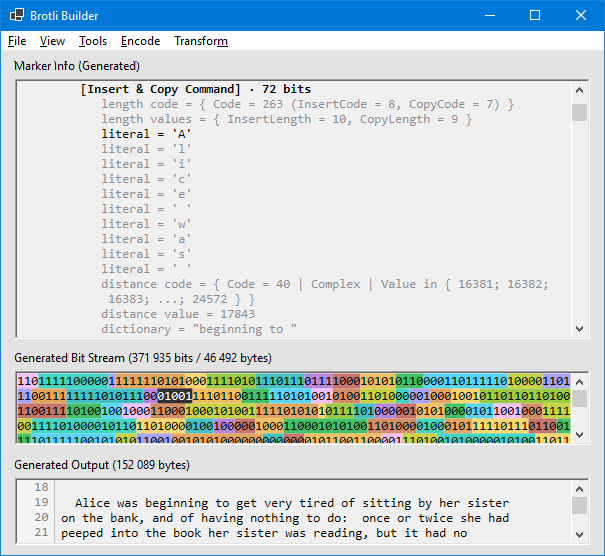
\includegraphics{Figures/ExampleBitMarkerGUI.png}
		\caption[Example of marked bits in the GUI application.]{Example of marked bits in the GUI application. The image shows a sequence of bit highlighted in the \texttt{Bit Stream} panel, and its label highlighted in the \texttt{Marker Info} panel. The bit sequence encodes the literal \enquote*{A}, as part of an insert\&copy command that produces the text \enquote{Alice\,\textvisiblespace \,was\,\textvisiblespace \,beginning\,\textvisiblespace \,to\,\textvisiblespace}.}
	\end{figure}
	
	\subsection{Decompression}
	
	The standard decompression algorithm produces uncompressed data as it reads and decodes each meta-block. In the custom implementation, we generate an object representation of each meta-block in which the data is already decoded, therefore we only have to extract it from the meta-blocks.
	
	All four meta-block types define a \verb|Decompress| method that takes a \verb|BrotliGlobalState| object, which --- as mentioned at the beginning of section \ref{sec:implementing-brotli} --- handles all state and output. Its default output processor only keeps uncompressed data the size of the sliding window, but we can choose to use an output processor that keeps all uncompressed data.
	
	To decompress a \verb|BrotliFileStructure|, initialize a \verb|BrotliGlobalState| with the custom output processor. Then for each meta-block, call the \verb|Decompress| method which works as follows:
	
	\begin{itemize} \nosep
		\item \textbf{Empty} meta-blocks output nothing
		\item \textbf{Uncompressed} meta-blocks output their uncompressed bytes
		\item \textbf{Compressed} meta-blocks do the following for each insert\&copy command:
			\begin{enumerate} \nosep
				\item Output all literals
				\item If the command has a \emph{copy} part, determine its type based on the current state:
					\begin{itemize}
						\item A backward reference outputs the byte at position given by $distance$ in a loop repeated $copy\ length$ times
						\item A dictionary reference unpacks the word index and transform ID from $distance$, reads the word using $copy\ length$ and word index, transforms it, and outputs it
					\end{itemize}
			\end{enumerate}
	\end{itemize}
	
	\subsection{Serialization}
	\label{sec:serialization}
	
	Serialization is defined similarly to deserialization. All component classes define a serialization procedure, which encodes each component into a \verb|BitWriter| --- the counterpart of \verb|BitReader| --- often also requiring a context object. Some components depend on an additional parameter object of type \verb|BrotliSerializationParameters|.
	
	The need for a special parameter object comes from the fact that several components of the Brotli format can be encoded into the bit stream in multiple valid ways. Finding the most optimal encoding is often impractical due to the sheer amount of combinations. Instead, developers come up with heuristics that find a good-enough solution to these kinds of problems. The parameter object is a set of user-provided heuristics (\verb|C#| function delegates) that make decisions about how to encode certain components.
	
	As the Brotli specification only explains the decoding process, all serialization procedures were reverse-engineered\footnote{Some heuristics from the official compressor were adapted into the library afterwards and are present in the current version, partly to allow for experimentation with parts of the official implementation, partly to retain \emph{some} consistency with the official implementation as the default behavior.} from descriptions of the format \& decoding algorithm. Naturally, this resulted in differences between files created by the official compressor, and the same files after they were deserialized and serialized again using the library.
	
	The following sections will explore components where these differences emerged, explain their bit representation and serialization procedure, and compare the custom and official implementation on the test corpus. We will skip components whose bit representation is unambiguous, as their serialization process usually involves simple calculations and/or lookup tables.\footnote{The official compressor employs many optimizations and arcane-looking computations for performance reasons. The custom implementation's source code favors simplicity over performance.}
	
	An important point is that serialization needs a fully defined \verb|BrotliFileStructure| object,\footnote{The streaming APIs do not need all meta-blocks at once, but they do need \texttt{BrotliFileParameters}, \texttt{BrotliGlobalState}, and a fully defined meta-block object.} where each meta-block header has all the necessary information to encode that meta-block's data. It is not allowed to modify any components.\footnote{The library guarantees that for any valid \texttt{BrotliFileStructure} or individual component class, serializing and then deserializing it yields an identical copy of it.} If, for example, an insert\&copy command encoded the literals \verb|abc| but \enquote*{c} was missing in the relevant Huffman tree, the serialization procedure would throw an exception --- the only way to resolve the issue would have involved modifying the Huffman tree to add the missing symbol, which is prohibited. Section \ref{sec:rebuilding-structure} will explore ways of (re)generating headers for new or modified meta-blocks.
	
		\subsubsection{Serializing Insert\&Copy Commands}
		\label{sec:serializing-ic-commands}
		
		Let us repeat what parts an insert\&copy command is made of, and add a few previously omitted details. An insert\&copy command begins with a \textbf{length code}, which encodes three parameters:
		
		\begin{itemize} \nosep
			\item Insert length (using an intermediary \emph{insert code})
			\item Copy length (using an intermediary \emph{copy code})
			\item Whether the \emph{implicit distance code zero} (\verb|IDCZ|) mark is present
		\end{itemize}
		
		\noindent
		The length code is immediately followed by an amount of \textbf{literals} equal to the insert length. Afterwards, one of the following situations happens:
		
		\begin{itemize} \nosep
			\item If the meta-block expects no more output, the command has no \emph{copy} part and the meta-block is terminated.
			\item If the \verb|IDCZ| mark is present, the command uses \textbf{distance code zero} --- which repeats the previous distance --- without reading anything from the bit stream.
			\item Otherwise, the command ends with an explicit \textbf{distance code} in the bit stream, which encodes the concrete distance.
		\end{itemize}
		
		\noindent
		The \textbf{length codes}, \textbf{distance codes}, and \textbf{literals} are the 3 main categories of symbols represented by Huffman trees. In the bit stream, any of these symbols may be preceded by a block-switch command.
		
		As mentioned previously, commands only keep the decoded data --- they do not remember which codes were used to encode that data. To serialize the 3 main categories of symbols, we proceed as follows:
		
		\begin{itemize} \nosep
			\item When writing the lengths, the Huffman tree is searched breadth-first for a length code that can encode the lengths and the \verb|IDCZ| mark. Only one such code can exist.
			\item When writing a literal, the Huffman tree is searched using a fast lookup structure, which directly maps literals to their paths in the tree.
			\item When writing the distance, we must remember that (1) some codes refer to previously seen distances, and (2) some consume a known amount of additional bits from the bit stream. Consequently, we have to consider two factors:
				\begin{enumerate} \nosep
					\item Multiple codes may be able to represent the same value.
					\item A code, which has the shortest path in the tree, may not actually be the most efficient if it requires additional bits.
				\end{enumerate}
			To find the shortest distance code, the Huffman tree is searched for all codes that can encode the concrete distance, and the one for which $(path\ length + additional\ bit\ count)$ is the smallest is chosen.
		\end{itemize}
		
		\noindent
		The laid out logic always finds the most efficient command encoding for a given meta-block header. In contrast, the official compressor immediately assigns length codes and distance codes as it generates the commands. It also tweaks path lengths of symbols in Huffman trees to take better advantage of special run-length codes that will explained in section \ref{sec:serializing-huffman-trees}, but at the expense of making some symbols take more bits. As a result, the official compressor does not always pick the most compact distance code, whereas the custom implementation sees the whole meta-block at once, allowing it to make better decisions when picking distance codes.
		
			\subfoursection{Distance Code Picking Comparison}
			
			The 169 test files compressed using 12 quality settings contained $200\,886\,450$ distance codes. The custom implementation chose a shorter distance code in $152\,582$ ($\approx 0.076 \%$) cases, in total saving $238\,986$ bits ($\approx$ \verb|29.17 KiB| or $0.0032 \%$ of the compressed corpus). Figure \ref{fig:serialization-savings-ic-commands} shows absolute savings by quality level.
			
			\begin{figure}[H]
				\centering
				\tikzfigure{reserialize-distance-code-savings}
				\smallskip
				\caption{Savings from custom implementation's more efficient distance code picking.}
				\label{fig:serialization-savings-ic-commands}
			\end{figure}
			
			\noindent
			When searching for codes that can encode a certain distance, the final list will always contain exactly 1 \textbf{direct} or \textbf{complex} code, and 0--4 \textbf{last} codes.
			
			The reason for no savings in quality levels 0 and 1 is that out of the 16 possible \textbf{last} codes, these quality levels only use code zero which repeats the last distance as-is. We will talk about code zero in section \ref{sec:building-insert-copy-commands}, but for now it is important to know that the decision to use (or not use) code zero in a command is set in stone, and cannot be changed during serialization.
			
			Although this shows a potential for improvements in the official compressor, the savings are minuscule and likely not worth the development attention that could be used elsewhere.
		
		\subsubsection{Serializing Block-Switch Commands}
		\label{sec:serializing-bs-commands}
		
		A block-switch command sets the current block type and new counter value for one of the 3 categories of symbols in insert\&copy commands. The block type and length are determined using a block type code and block length code respectively. Both codes are stored using Huffman trees, but block length codes are unambiguous so this section will not pay attention to them.
		
		Each category can define up to 256 distinct block types per meta-block. The Huffman tree alphabet for type codes has 258 symbols --- the first 2 symbols refer to previously seen block types, the remaining 256 symbols map directly to the 256 possible block types.
		
		Block type codes do not require any additional bits unlike distance codes, so a breadth-first search of the Huffman tree is sufficient to find the most compact one. In contrast, the official compressor tests block type codes in a fixed order at the time it generates the command.
		
			\subfoursection{Block Type Code Picking Comparison}
			
			The 169 test files compressed using 8 highest quality settings --- those which perform block splitting --- contained $303\,725$ block-switch commands. The custom implementation chose a shorter block type code in $5\,560$ ($\approx 1.83 \%$) cases, in total saving $8\,507$ bits ($\approx$ \verb|1.04 KiB| or $0.00012 \%$ of the compressed corpus). Figure \ref{fig:serialization-savings-bs-commands} shows absolute savings per quality level:
			
			\begin{figure}[H]
				\centering
				\tikzfigure{reserialize-block-type-code-savings}
				\smallskip
				\caption{Savings from custom implementation's more efficient block type code picking.}
				\label{fig:serialization-savings-bs-commands}
			\end{figure}
		
		\subsubsection{Serializing Context Maps}
		
		A context map maps every possible \pair{block\ type}{context\ ID} pair to an index in an array of Huffman trees. Each meta-block header defines one context map for literals (64 context IDs) and one context map for distance codes (4 context IDs). The mapping is implemented as a single byte array of size $(total\ block\ types \times total\ context\ IDs)$.
		
		In the bit stream, a context map begins with a variable-length code that reads a value between 1--256. This value indicates the amount of Huffman trees, which also tells us the size of the Huffman tree array, and the range of indices that can appear in the context map data.
		
		If the amount of Huffman trees equals 1, the context map is \emph{trivial} --- all indices are zero. Otherwise, we have to reconstruct the entire byte array, which may span up to $256 \times 64$ elements or \verb|16 KiB| for literals, and $256 \times 4$ elements or \verb|1 KiB| for distance codes. Storing the entire array as a contiguous sequence of bytes would be highly inefficient (see figure \ref{fig:test-corpus-context-map-bits} in the next section). Predictably, Brotli employs several techniques to greatly compact them.
		
		Firstly, we can encode the array of bytes using a Huffman tree with symbols 0--255, denoting their respective byte values. This also lets us omit unused symbols, yielding significant savings in meta-blocks with small amounts of Huffman trees.
		
		Secondly, presume that context maps will have consecutive occurrences of the same value, also called \emph{runs}. For example, we could assign a separate Huffman tree to each block type. Figure \ref{fig:context-map-long-runs} shows such context map for literals with 3 block types, resulting in 3 runs of 64 values each:
		
		\begin{figure}[H]
			\centering
			$\underbrace{0,\dots,0}_{64 \times},\underbrace{1,\dots,1}_{64 \times},\underbrace{2,\dots,2}_{64 \times}$
			\caption{Example context map with long runs.}
			\label{fig:context-map-long-runs}
		\end{figure}
		
		\noindent
		Brotli heavily optimizes these kinds of context maps by combining two general compression techniques:
		
		\begin{enumerate} \nosep
			\item \textbf{Move-to-front transform} takes a set alphabet, but instead of encoding the symbols, it encodes each symbol's ordinal in the alphabet --- then, that symbol is moved to the first position (front) in the alphabet\cite{DataCompressionCompleteReference}. See table \ref{table:move-to-front-english-word} for an example of applying the move-to-front transform to an English word, and pay attention to low numbers where letters repeat.\footnote{One possible way to exploit this would be to use Huffman coding, assigning short bit sequences to low numbers and long bit sequences to high numbers.}
			
			During serialization, Brotli applies the move-to-front transform on the context map byte array, whose alphabet consists of the byte values 0--255. During deserialization, it uses an inverse transform described in the Brotli specification to retrieve the original values. Although Brotli makes the transform optional, the official compressor enables it in all context maps.
			
			\begin{table}[H]
				\centering
				\medskip
				\caption[Example of applying the move-to-front transform in individual steps.]{Example of applying the move-to-front transform in individual steps. The alphabet consists of English letters \texttt{a-z} where \texttt{a = 1} and \texttt{z = 26}.}
				\label{table:move-to-front-english-word}
				\texfigure{move-to-front-english-example}
			\end{table}
			
			\noindent
			Figure \ref{fig:move-to-front-context-map} is an example of a small context map for distances, which uses a separate Huffman tree for each of its 3 block types. The figure shows its values before and after applying the move-to-front transform, turning it from a sequence where all values have equal probability into a sequence where $0$ is the most frequent.
			
			\begin{figure}[H]
				\centering
				\smallskip
				$0, 0, 0, 0, 1, 1, 1, 1, 2, 2, 2, 2$
				\\
				$\downarrow$
				\\
				$0, 0, 0, 0, 1, 0, 0, 0, 2, 0, 0, 0$
				\caption{Example of applying the move-to-front transform to a context map.}
				\label{fig:move-to-front-context-map}
			\end{figure}
			
			\item \textbf{Run-length encoding}\cite{DataCompressionCompleteReference} replaces consecutive occurrences of the same symbol --- runs --- with an instruction that encodes only one instance of the symbol, and the amount of its occurrences --- run length.
			
			In context maps, Brotli uses run-length encoding for runs of the symbol $0$. Non-trivial context maps have a parameter which adds up to 16 intermediary codes into the alphabet of byte values, potentially expanding the alphabet from 256 to 272 symbols. As is usual with intermediary codes, each code can represent a range of run lengths, and consumes additional bits to find the offset within that range.
			
			If all 16 codes are used, the maximum representable run length is $2^{17} - 1 = 131\,071$. However, $16\,383$ is the longest run actually possible in Brotli,\footnote{A context map for literals with 256 block types would contain $256 \times 64 = 16\,384$ values. The longest run is one less because at least one value must differ --- otherwise it would be treated as a trivial context map.} which matches the maximum run length of code 13 ($2^{14} - 1$).
			
			In practice, most context maps generated by the official compressor are either similar to the one in figure \ref{fig:move-to-front-context-map}, or they are generated from statistics about the input file and those do not normally end up with very long runs.
		\end{enumerate}
		
			\subfoursection{Optimization Analysis}
			
			Let us digress for a moment to test the usefulness of Huffman coding, move-to-front transform, and run-length encoding in context maps across the test corpus.
			
			From all compressed files, information about every non-trivial context map was compiled into a single list. Figure \ref{fig:test-corpus-context-map-bits} shows a ratio for each quality level. The ratio was calculated as the sum of all actually used bits, divided by the amount of bits all byte arrays would use if encoded raw.\footnote{The actually used bits include the Huffman tree and other metadata needed to decode the context map. If context maps were encoded as raw byte arrays, they would not need this metadata, thus the comparison is fair.} The increasing ratio --- decreasing effectiveness --- correlates with increasing complexity of context maps in high quality levels.
			
			\begin{figure}[H]
				\centering
				\tikzfigure{test-corpus-context-map-bits}
				\caption{Analysis of context map optimization effectiveness across test corpus files.}
				\label{fig:test-corpus-context-map-bits}
			\end{figure}
		
			\subfoursection{Serialization Parameters}
			When tasked with serializing a context map, we have a few decisions to make:
			
			\begin{itemize} \nosep
				\item Do we apply the move-to-front transform?
				\item What is the best way of encoding each run? Should we use special codes at all?
				\item What is the best way of encoding the Huffman tree for byte values and special codes?
			\end{itemize}
			
			\noindent
			Let us consider two tricky scenarios.
			
			\begin{enumerate} \nosep
				\item The sequence $(0, 0, 0, 1)$ has a run replaceable by a special code, reducing its size by 1. However, enabling special codes for the context map uses 4 extra bits, and expands the Huffman tree alphabet which in this case adds 2 bits. Our net \enquote{savings} are $-5$ bits.
				\item A run of 8 zeros is at a boundary --- the run is completely covered by special code 3, but can also be encoded using special code 2 followed by a single 0. Which option is better depends on their paths in the Huffman tree, and the encoding of the Huffman tree itself.
			\end{enumerate}
			
			\noindent
			All decisions are ultimately passed onto the library user with \verb|BrotliSerializationParameters|. Context maps serialization defines three parameters --- function delegates. The move-to-front parameter takes a context map, and returns a boolean that says whether to use the transform. The run-length parameter is given all runs found in the byte array, and a system to accept/reject/split each one. The Huffman tree parameter takes a list of symbol frequencies and returns the tree structure.
			
			The defaults are set to always use move-to-front, replace every run with a special code that fully covers it, and use the classic Huffman coding algorithm to generate the tree.
			
			\subfoursection{Comparison}
			
			This comparison tests combinations of strategies on the test corpus. It is important to acknowledge the limits of this exercise --- we are evaluating  strategies with fixed rules, and only on context maps generated by the official compressor. The best overall strategy we find will certainly not be the best for all possible context maps. Huffman trees are also a factor --- their serialization will be discussed in section \ref{sec:serializing-huffman-trees}, but they do mildly differ from the official compressor.
			
			The data was obtained by individually serializing all non-trivial context maps in the test corpus and counting the bits. Figures \ref{fig:reserialize-context-map-strategies-literal-best} and \ref{fig:reserialize-context-map-strategies-distance-best} show the total amounts of bits for each quality level. Tables \ref{table:reserialize-context-map-strategies-literal-best} and \ref{table:reserialize-context-map-strategies-distance-best} note which strategies encoded context maps the best, and which were tied with another strategy. All combinations of the following parameters were tested:
			
			\begin{itemize} \nosep
				\item \textbf{MTF} (move-to-front transform)
					\begin{itemize} \nosep
						\item \textbf{Yes} enables the transform
						\item \textbf{No} disables the transform
					\end{itemize}
				\item \textbf{RLE} (run-length encoding)
					\begin{itemize} \nosep
						\item \textbf{No} does not use special codes
						\item \textbf{Full} encodes all runs using special codes
						\item \textbf{Split} encodes all runs using special codes, but if shortening the run by 1 also shortens the code, it encodes the shorter run followed by a plain 0
					\end{itemize}
			\end{itemize}
			
			\noindent
			The results indicate that using the move-to-front transform is in almost all cases the best option, but it does lose some effectiveness in the two highest quality levels that generate the most complex context maps. There is no single run-length encoding strategy that works best in all quality levels and types of context maps, but choosing either \textbf{Full} or \textbf{Split} strategy yields sufficiently good results.
			
			\pagebreak
			
			\begin{table}[H]
				\centering
				\caption{\% of times a strategy for non-trivial context maps for literals was the best/tied.}
				\label{table:reserialize-context-map-strategies-literal-best}
				\texfigure{reserialize-context-map-strategies-literal-best}
			\end{table}
			\vfill
			\begin{figure}[H]
				\centering
				\tikzfigure{reserialize-context-map-strategies-literal}
				\\[-0pt]
				\caption{Comparison of serialization strategies in non-trivial context maps for literals.}
				\label{fig:reserialize-context-map-strategies-literal-best}
			\end{figure}
			
			\pagebreak
			
			\begin{table}[H]
				\centering
				\caption{\% of times a strategy for non-trivial context maps for distance codes was the best/tied.}
				\label{table:reserialize-context-map-strategies-distance-best}
				\texfigure{reserialize-context-map-strategies-distance-best}
			\end{table}
			\vfill
			\begin{figure}[H]
				\centering
				\tikzfigure{reserialize-context-map-strategies-distance}
				\\[-0pt]
				\caption{Comparison of serialization strategies in non-trivial context maps for distance codes.}
				\label{fig:reserialize-context-map-strategies-distance-best}
			\end{figure}
			
		\subsubsection{Serializing Huffman Trees}
		\label{sec:serializing-huffman-trees}
		
		The Brotli format has two ways to encode Huffman trees --- \textbf{simple} and \textbf{complex}. The \textbf{simple} encoding handles trees with 1--4 symbols, in five possible shapes displayed in figure \ref{fig:huffman-tree-simple-shapes}. A tree with only 1 symbol is a special case, where reading the symbol does not consume any bits from the bit stream.
		
		\begin{figure}[H]
			\centering
			\medskip
			\tikzfigure{huffman-tree-simple-shapes}
			\medskip
			\caption{Shapes of Huffman trees that can use the simple form of encoding.}
			\label{fig:huffman-tree-simple-shapes}
		\end{figure}
		
		\noindent
		The \textbf{complex} form is based on canonical Huffman coding\cite{RFC7932}, which is also used by other compression standards such as DEFLATE\cite{RFC1951}.
		
		Canonical Huffman coding only stores the path lengths of each symbol, following the order in which the symbols appear in the alphabet. Brotli does two things to condense them even further. Firstly, it uses special codes as a form of run-length encoding:
		
		\begin{itemize} \nosep
			\item \textbf{Code 0} means the current symbol is not present in the tree
			\item \textbf{Codes 1--15} assign the current symbol a path length of 1--15
			\item \textbf{Code 16} repeats the last assigned path length over the next several symbols
			\item \textbf{Code 17} repeats code 0 over the next several symbols, efficiently skipping unused symbols in large alphabets
		\end{itemize}
		
		\noindent
		Secondly, these codes are read with the help of a \emph{secondary} Huffman tree, which is freshly generated for each \emph{primary} tree. The secondary tree is also stored using canonical Huffman coding, and its own path lengths are stored with a variable-length code defined in the Brotli specification.
		
		Codes 16 and 17 are followed by 2 and 3 extra bits respectively, which are used in the computation of the run length. When a repetition code itself repeats, the previously read extra bits act as a multiplier of the current result. This is best shown on an example of code 16's first several run lengths and how they are represented:
		
		\begin{figure}[H]
			\centering
			\texfigure{huffman-tree-code-16-example}
			\caption{Computing run lengths from repeated code 16 \& extra bits in Huffman tree serialization.}
		\end{figure}
		
		\noindent
		The custom implementation includes the classic Huffman coding algorithm based on symbol frequencies, and also the canonical Huffman coding algorithm. Brotli additionally imposes a depth limit --- primary trees must have path lengths of at most 15, secondary trees at most 5. In the custom implementation, depth-limiting uses a heuristical approach described by Charles Bloom, although solving the problem optimally is possible using the package-merge algorithm\cite{DepthLimitedHuffmanTrees}.
		
			\subfoursection{Serialization Parameters}
			
			The amount and complexity of Huffman trees make them the bulk of meta-block headers --- across the test corpus, they make up $\approx 94.4 \%$ of all header bits.
			
			\verb|BrotliSerializationParameters| exposes two parameters --- function delegates. Similarly to context maps, one parameter controls run-length encoding --- this time in terms of codes 16 and 17 --- by asking the parameter how to handle each run in the sequence, and one parameter controls generation of the secondary Huffman tree. By default, the library encodes runs using a heuristic adapted from the official compressor:
			
			\begin{itemize} \nosep
				\item If the tree's symbol alphabet contains 50 symbols or fewer, run-length encoding is skipped
				\item Code 16 is used for runs of non-zero codes if $\sum_{i=1}^n{length_i} > 2n$, for $length_i \geq 4$
				\item Code 17 is used for runs of zeros if $\sum_{i=1}^n{length_i} > 2n$
				\item Code 16 runs of length 7 are split\footnote{The last 2 rules are special cases for the first run lengths that require 2 successive repetition codes. The heuristic assumes it is always better to encode one of the symbols normally and reduce the run length by one.} into 1 normal code and a run of length 6
				\item Code 17 runs of length 11 are split\footnote{See previous footnote.} into 1 normal code and a run of length 10
			\end{itemize}
			
			\noindent
			Using the same heuristic makes Huffman tree encoding nearly identical to the official compressor. A difference still exists in generation of the secondary tree --- one interesting optimization the official compressor applies to some trees is equalizing adjacent symbols' path lengths to form longer runs. This condenses the meta-block header at the expense of using more bits in the data section, as the tree is no longer optimal. Such optimization could be reimplemented using the parameters that control how Huffman trees are generated --- that would affect secondary trees mentioned in this section, and trees generated for context map values. In order to apply this optimization to other Huffman trees, such as the ones for insert\&copy command elements, we would have to rebuild the meta-block header, which will be discussed in section \ref{sec:rebuilding-structure}.
			
		\subsubsection{Concluding Serialization}
		
		This section takes a brief look at the overall differences in compressed size between the custom and official implementations. To reiterate an important point, serialization is not allowed to modify data in any of the components, it does however regenerate metadata about how certain components are encoded in the bit stream.
		
		Figure \ref{fig:reserialize-overall-comparison} shows the differences after taking every file from the test corpus, deserializing it, and serializing it again with default \verb|BrotliSerializationParameters|. To eliminate outliers, files whose uncompressed size was less than \verb|512 B| were excluded (8 files in total). Plot whiskers show the minimum and maximum. The second plot zooms in on quality levels 3--11.
		
		\begin{figure}[H]
			\tikzfigure{reserialize-overall-comparison}
			\\[-0pt]
			\tikzfigure{reserialize-overall-comparison-zoomed}
			\vspace{0pt}
			\caption{Compressed file size ratios (custom serialization $\div$ official implementation).}
			\label{fig:reserialize-overall-comparison}
		\end{figure}
		
		\noindent
		Largest improvements are found in quality levels 0--2, mainly because the secondary trees they use to encode Huffman trees are predefined, while the custom implementation generates them from scratch. Low quality levels also tend to generate higher quantities of shorter meta-blocks, giving the custom implementation more Huffman trees --- opportunities --- to optimize.
	
	\subsection{(Re)building the Structure}
	\label{sec:rebuilding-structure}
	
	Although serialization is a crucial part of supporting the Brotli format, we want the ability to modify an existing \verb|BrotliFileStructure| or create a completely new one. The library streamlines this process, making it less error-prone than if we tried to do it manually.
	
	This section introduces several builder APIs that automate construction of meta-block header components --- such as Huffman trees and codes used in commands --- from the data we want to encode. We will go over examples of using the API, and some implementation details of the builders and related utilities.
	
		\subsubsection{Dictionary Implementation}
		
		A \verb|BrotliDictionary| definition consists of 3 parts:
		
		\begin{itemize} \nosep
			\item \textbf{Data source} that can seek and retrieve the raw bytes that form dictionary words. A~source can be a file or data stream, or even a simple byte array in memory.
			\item \textbf{Word transforms} that govern how prefixes, suffixes, and transforms are applied to the retrieved words, as described in section \ref{sec:dictionary-word-transformations}.
			\item \textbf{Format definition} that describes the data source's structure, knows how to locate words in the data source by their length and index, and packs/unpacks the word index and transform ID to/from dictionary references.
		\end{itemize}
		
		\noindent
		The default dictionary sets the format and word transforms according to the standard, and its data source is a file embedded into the library.
		
		Note that while the library makes it possible to use custom dictionaries, it would be up to the user to remember which dictionary was used for which files, and ensure their data sources are available to perform decompression. For that reason, and because the upcoming Brotli format extension would require additional changes for proper support, the library's current implementation of custom dictionaries is not particularly useful for real-world use cases.
		
			\subfoursection{Index Structure}
			
			An index structure finds dictionary references that match the beginning of a given sequence of bytes. A dictionary reference takes the form of a \pair{copy\ length}{packed\ value} pair.
			
			Internally, the index uses PATRICIA trees. This type of tree was chosen because it has the interface of prefix trees --- unlike for example a hash table --- and it is much more compact in memory than a classic \emph{trie}. A prefix tree interface matches on a common prefix. We can take an arbitrarily long sequence of bytes, traverse down the tree and at each node add matching entries to a list, and end up with a collection of all dictionary references matching the beginning of the sequence.
			
			For example, let us search the phrase \enquote{Back to the future} for matches at least 4 bytes long. Figure \ref{fig:dictionary-index-lookup-example} shows gradual matches for all prefixes of the phrase, assuming a scenario in which the entire dictionary --- including all transformed words --- is stored in a single tree. The end of each row lists matching \triple{word\ length\ group}{word\ index}{transform\ ID} triples.
			
			\begin{figure}[H]
				\texfigure{dictionary-index-lookup-example}
				\caption{Results of dictionary index lookup on prefixes of the input of length $\geq 4$.}
				\label{fig:dictionary-index-lookup-example}
			\end{figure}
			
			\noindent
			We can look at some of the results to find out how they work:
			
			\begin{itemize} \nosep
				\item \triple{4}{4}{9}\,:\,Word 4 of length 4 is \verb|back|, transform 9 makes it \verb|Back|
				\item \triple{4}{4}{4}\,:\,Word 4 of length 4 is \verb|back|, transform 4 makes it \texttt{Back\textvisiblespace}
				\item \triple{10}{86}{56}\,:\,Word 86 of length 10 is \verb|Background|, transform 56 makes it \verb|Back|
				\item \triple{12}{397}{9}\,:\,Word 397 of length 12 is \texttt{back\textvisiblespace to\textvisiblespace the\textvisiblespace}, transform 9 makes it  \texttt{Back\textvisiblespace to\textvisiblespace the\textvisiblespace}
			\end{itemize}
			
			\noindent
			All findings are made available to the caller, so that they can decide which one to pick --- longest matches are not always advantageous, as increasing word lengths and especially large transform IDs can greatly inflate distances in insert\&copy commands, needing more bits to encode.
			
			A naïve way to construct the index may iterate through all 121 word transforms, apply each to all words in the dictionary, and store everything in a single tree. Although the dictionary index is constructed lazily at first request, even that first request should be reasonably fast, which requires a smarter approach.
			
			Instead, there is a separate PATRICIA tree for each of the 21 preset functions --- recall those are \textbf{Identity}, \textbf{Omit First 1--9}, \textbf{Omit Last 1--9}, \textbf{Ferment First}, and \textbf{Ferment All}. The functions are one by one applied to each word in the dictionary, then words with at least 1 byte remaining are stored in the corresponding tree. Notice that prefixes and suffixes are not included in the trees, so they must be accounted for during lookup instead. The lookup procedure works as follows:
			
			\begin{enumerate} \nosep
				\item Consider only transforms which have no prefix, or whose prefix matches the beginning of the searched input.
				\item For each transform, strip its prefix from the input, then perform lookup in the tree assigned to the transform's function.\footnote{Many transforms use the same function, so the tree lookup can be memoized.}
				\item For each match, strip the transformed word from the input, and ensure the rest matches the transform's suffix.
				\item Return all valid matches.
			\end{enumerate}
			
			\noindent
			A match comprises the dictionary reference \pair{copy\ length}{packed\ value} as well as the actual output length to help us select the best result. To construct an insert\&copy command, we must know the sliding window size, and the amount of bytes output at the exact point this command will be read. If we are adding literals into the command, they must also be counted. The final distance is: $packed\ value + 1 + \min (window\ size,\ output\ size + amount\ of\ literals)$.
		
		\subsubsection{Building Insert\&Copy Commands}
		\label{sec:building-insert-copy-commands}
		
		\verb|CompressedMetaBlockBuilder| is a builder API for creating and editing meta-blocks. It takes an initial \verb|BrotliGlobalState| that describes the state at the beginning of this meta-block, and optionally an existing meta-block from which it copies the header and data. Figure \ref{fig:compressed-meta-block-components-reminder} is a reminder about all components of a compressed meta-block.
		
		\begin{figure}[H]
			\centering
			\medskip
			
			\begin{tabular}{lcl}
				\textbf{Header} & & \textbf{Data} \\
				\addlinespace
				\cline{1-1} \cline{3-3}
				\addlinespace
				Block Type Info $\times$ \verb|[L,I,D]|    & & List of Insert\&Copy Commands \\
				Distance Parameters                        & & List of Block-Switch Commands $\times$ \verb|[L,I,D]| \\
				Literal Context Mode Array                 & & \\
				Context Map $\times$ \verb|[L,D]|          & & \\
				Huffman Tree Array $\times$ \verb|[L,I,D]| & & \\
			\end{tabular}
			
			\caption{Compressed meta-block header and data components.}
			\label{fig:compressed-meta-block-components-reminder}
		\end{figure}
		
		\noindent
		Building block-switch commands and information about block types and lengths will be covered in section \ref{sec:building-block-switch-commands}, and context maps in section \ref{sec:building-context-maps}. Distance parameters and literal context modes are exposed as read/write properties. The job of a \verb|CompressedMetaBlockBuilder| is to process insert\&copy commands, generate Huffman tree arrays based on the commands and other header parameters, and combine everything into the final meta-block object.
		
		Listing \ref{lst:meta-block-builder-api-examples} is a \verb|C#| code snippet that creates a meta-block from scratch using the builder API.
		
		\lstinputlisting[
			label = {lst:meta-block-builder-api-examples},
			caption = {\texttt{CompressedMetaBlockBuilder} API usage examples.}
		]{SourceCodes/CompressedMetaBlockBuilderAPI.cs}
		
		\noindent
		As commands are added, the builder tracks the transitional state so that it (1) knows how many bytes were output so far, (2) remembers the previous distance to substitute matching distances with distance code 0, and (3) calculates distances for dictionary references.
		
		Distance code 0 is treated specially --- it does not update the buffer of previously used distances, and it can sometimes be encoded directly in the command length code (the \verb|IDCZ| mark). The library handles special cases concerning distances with an enumeration type \verb|DistanceInfo|, whose instances are either positive integers denoting concrete distances, or one of 3 special values:
		
		\begin{itemize} \nosep
			\item \verb|EndsAfterLiterals|
			\item \verb|ImplicitCodeZero|
			\item \verb|ExplicitCodeZero|
		\end{itemize}
		
		\noindent
		This is why decisions about using code 0 are made during command creation. Builder methods that take concrete distances have an optional parameter which, if the passed distance is the same as the previous distance, decides whether to use an implicit code zero, explicit code zero, or encode the distance without code zero. The default behavior is to use implicit code zero if possible, explicit code zero otherwise.
		
		Once all commands and customizable header components are set, the build process can begin:
		
		\begin{enumerate} \nosep
			\item Build block-switch commands (section \ref{sec:building-block-switch-commands})
			\item Determine sizes of the Huffman tree arrays:
				\begin{itemize} \nosep
					\item For length codes, the size equals the amount of block types for length codes
					\item For literals and distance codes, sizes are set in context maps
				\end{itemize}
			\item Initialize a symbol frequency counter for each Huffman tree index
			\item Simulate all insert\&copy and block-switch commands:
				\begin{itemize} \nosep
					\item Determine next block type ($=$ tree index) for length codes
					\item Generate the length code and add it to the frequency counter
					\item For each literal:
						\begin{itemize} \nosep
							\item Determine next block type for literals
							\item Determine next tree index for literals
							\item Add literal to the frequency counter
						\end{itemize}
					\item If the command has an explicit distance:
						\begin{itemize} \nosep
							\item Determine next block type for distance codes
							\item Determine next tree index for distance codes
							\item Generate the distance code and add it to the frequency counter
						\end{itemize}
				\end{itemize}
			\item Convert all symbol frequency counters into Huffman trees
			\item Return the meta-block, and the final state object that can be fed into the next builder
		\end{enumerate}
		
		\noindent
		Length \& distance code generation can be optimized to various degrees. The most basic implementation could iterate all codes and check which values each can encode. The official implementation pushes for performance by combining patterns in the encodable values with arithmetic and bitwise operations. The custom implementation sits somewhere in the middle.
		
		As with serialization, we can provide a parameter object --- \verb|BrotliCompressionParameters|. Here, it controls the generation of Huffman trees, and decides which distance code to pick if multiple valid options are available. By default, Huffman trees use the classic Huffman coding algorithm, and distance code picking will be explored in the next section.
		
		Codes generated in the build process determine which codes become available in Huffman trees and how many bits they take. It is then up to serialization to look at each symbol, and pick the best code for it from the generated Huffman trees. This also applies to codes and values generated by block-switch builders.
		
			\subfoursection{Distance Code Picking Analysis}
			
			The distance code picker parameter is a function delegate called any time a distance can be written using two or more codes. It takes a list of candidate codes and frequencies of previously picked codes, and produces one code to add into the Huffman tree. Candidates are ordered by their position in the distance code symbol alphabet, which means that \textbf{Last} codes --- those that refer to previous distances --- always come first, and they are always followed by one either \textbf{Direct} or \textbf{Complex} code (both cannot refer to the same distance at once). We can try a few picking strategies:
			
			\begin{itemize} \nosep
				\item \textbf{First Option} is the default. It picks the first candidate, which is always a \textbf{Last} code.
				\item \textbf{Seen} picks the first candidate that had been picked before, or the first candidate if none have been picked before.
				\item \textbf{Frequent} picks the candidate that has been picked the most frequently so far, or the first candidate if none have been picked before.
				\item \textbf{Non-Last} picks the candidate which is not a \textbf{Last} code.
			\end{itemize}
			
			\noindent
			Figure \ref{fig:picking-strategies-distance-codes} compares these strategies on the test corpus, using the \textbf{First} strategy as a baseline. Plot whiskers show the minimum and maximum.
			
			\begin{figure}[H]
				\centering
				\tikzfigure{picking-strategies-distance-codes}
				\\[-0pt]
				\caption{Comparison of distance code picking strategies on the test corpus.}
				\label{fig:picking-strategies-distance-codes}
			\end{figure}
		
		\subsubsection{Building Block-Switch Commands}
		\label{sec:building-block-switch-commands}
		
		A \verb|CompressedMetaBlockBuilder| allows configuring blocks and block-switch commands using a dedicated builder for each of the 3 categories of elements:
		
		\medskip
		\lstinputlisting[
			caption = {Obtaining block-switch builders from a \texttt{CompressedMetaBlockBuilder}.},
			emph = {Category}
		]{SourceCodes/BlockSwitchBuilderGetters.cs}
		\medskip
		
		\noindent
		The API is again best shown by example. The following listings and figures perform block splitting on a sequence of 11 insert\&copy command length codes. The first block always has a block type of 0, and its length is set using either \verb|SetInitialLength| or \verb|AddBlock| with type 0. If \verb|AddFinalBlock| is used, its length will cover all remaining symbols. Note that calling \verb|Reset| is not strictly necessary, but it ensures we start from a clean slate when modifying a meta-block.
		
		\begin{figure}[H]
			\medskip
			\texfigure{block-switch-builder-api}
			\caption{\texttt{BlockSwitchBuilder} API usage examples.}
			\medskip
		\end{figure}
		
		\noindent
		As mentioned in the previous section, block-switch commands are built when the meta-block is built. The build process for each block-switch builder works as follows:
		
		\begin{enumerate} \nosep
			\item Initialize two symbol frequency counters:
				\begin{itemize} \nosep
					\item One counts block type codes
					\item One counts block length codes, immediately counting a code that encodes the initial block length
				\end{itemize}
			\item Simulate all block-switch commands:
				\begin{itemize} \nosep
					\item Generate the type code and add it to the frequency counter
					\item If this is the last command and \verb|AddFinalBlockSwitch| was used, calculate the final block length
					\item Generate the length code and add it to the frequency counter
				\end{itemize}
		\end{enumerate}
		
		\noindent
		\verb|BrotliCompressionParameters| again controls the generation of Huffman trees, and one parameter also picks the block type code if multiple can be used.
		
			\subfoursection{Block Type Code Picking Analysis}
			The block type code picker parameter works exactly like the distance code picker. Brotli defines two special codes --- code 0 repeats the previous block type, code 1 increments the current block type and wraps around to $BT = 0$ if necessary.
			
			The code picker is only asked if multiple codes can be used, so for a block type $x$ the only possible candidate lists are $[\,0,\,x + 2\,]$, $[\,1,\,x + 2\,]$, or $[\,0,\,1,\,x + 2\,]$. The next test tries the following picking strategies:
			
			\begin{itemize} \nosep
				\item \textbf{Prefer Code 0} uses code 0 if available, otherwise uses the first candidate. This is the default strategy in the custom implementation.
				\item \textbf{Prefer Code 1} uses code 1 if available, otherwise uses the first candidate. This is how the official compressor behaves.
				\item \textbf{Non-Special} always picks the last candidate, avoiding both code 0 and 1.
			\end{itemize}
		
			\noindent
			Figure \ref{fig:picking-strategies-block-type-codes} compares these strategies on the test corpus, using \textbf{Prefer Code 0} as a baseline. Quality levels 0--3 do not perform block splitting and thus are excluded. Plot whiskers show the minimum and maximum.
			
			\begin{figure}[H]
				\centering
				\tikzfigure{picking-strategies-block-type-codes}
				\\[-0pt]
				\caption{Comparison of block type code picking strategies on the test corpus.}
				\label{fig:picking-strategies-block-type-codes}
			\end{figure}
		
		\subsubsection{Building Context Maps}
		\label{sec:building-context-maps}
		
		This section introduces an API that simplifies context map creation. First, we must know the amount of block types, then construct either \verb|ContextMapBuilder.Literals| or \verb|.Distances|. Listing \ref{lst:context-map-builder-api-examples} showcases how the API can be used to set the mapping for entire block types, individual indices, or ranges of indices.\footnote{Note that calling \texttt{RepeatFirstBlockType} without separating the trees creates a useless context map where all block types have the exact same tree indices. It could however be used to propagate a pattern across all block types and then start changing individual indices.} The context map array contents are shown below each API call, with asterisks indicating which positions were touched by that call.
		
		\medskip
		\lstinputlisting[
			label = {lst:context-map-builder-api-examples},
			caption = {\texttt{ContextMapBuilder} API usage examples.}
		]{SourceCodes/ContextMapBuilderAPI.cs}
		\medskip
		
		\noindent
		The built \verb|ContextMap| object stores the category (literals or distance codes), an immutable copy of the context map array, and the amount of Huffman trees calculated as $(1 + maximum\ value)$. For example, the context map from listing \ref{lst:context-map-builder-api-examples} would have 6 Huffman trees.
		
		\subsubsection{Final Comparison}
		
		This section applies the \textbf{rebuild} meta-block transformation to the test corpus. The transformation passes a meta-block to \verb|CompressedMetaBlockBuilder| and simply rebuilds it, causing all Huffman trees and codes the be regenerated. Figure \ref{fig:rebuild-overall-comparison} shows size ratios between files originating from the official compressor and the rebuilt ones. Plot whiskers show the minimum and maximum. The second plot zooms in on quality levels 3--11.
		
		\begin{figure}[H]
			\tikzfigure{rebuild-overall-comparison}
			\\[-0pt]
			\tikzfigure{rebuild-overall-comparison-zoomed}
			\vspace{0pt}
			\caption{Compressed file size ratios (custom builder $\div$ official implementation).}
			\label{fig:rebuild-overall-comparison}
		\end{figure}

\section{Official Implementation}
\label{sec:official-implementation}

This section focuses on the official compressor implementation. We will begin by summarizing differences between the quality levels (0--11). Then, we will delve into individual features, exploring their implementation and their effect on the test corpus. Finally, we will try experimenting with the source code in an attempt to find improvements.

	\subsection{Official Quality Levels}
	
		\subsubsection{Quality Levels 0--1}
		The two lowest quality levels are reimplementations of Google's high speed Snappy\footnote{\url{https://github.com/google/snappy}} compressor adapted to the Brotli format. Both qualities generate insert\&copy commands in an interesting way that reduces the amount of length codes defined in the header --- instead of generating one command with both the \emph{insert} and \emph{copy} part, it splits them into two commands.
		
		The first command is for the \emph{insert} part, and because every command must have a minimum copy length of 2, it also includes 2 bytes of the copy. The second command outputs the rest of the copy, using distance code zero as the distance is the same as that of the previous command.
		
		We can visualize the commands with an example. Figure \ref{fig:quality-0-1-command-generation-example} shows how one command generating the phrase \enquote{words, words} would be split into two.
		
		\begin{figure}[H]
			\medskip
			\texfigure{quality-0-1-command-generation-example}
			\caption{Insert\&copy command generation pattern in official compressor's lowest quality levels.}
			\label{fig:quality-0-1-command-generation-example}
		\end{figure}
		
		\noindent
		Instead of 704 length codes covering all possible combinations of \emph{insert} and \emph{copy} codes and \verb|IDCZ| marks, we merely have to account for the following cases covered by only 59 length codes:
		
		\begin{itemize} \nosep
			\item $(\,insert\ length > 0\ \wedge\ copy\ length = 2\,)$
			\item $(\,insert\ length = 0\ \wedge\ copy\ length \geq 2\,)$
			\item $(\,insert\ length = 0\ \wedge\ copy\ length \geq 2\ \wedge\,\mathtt{IDCZ}\,)$
		\end{itemize}
		
		\noindent
		This simplifies meta-block generation in both quality levels. Quality level 0 starts with predefined length \& distance code Huffman trees, which means those trees must include all possible codes, and it immediately begins outputting commands. If a second (third, fourth, etc.) meta-block is generated, it will use knowledge about the previous meta-block codes to adjust the length \& distance code trees. Quality level 1 and higher generate commands for a meta-block first, and construct trees based on the actual encoded data.
		
		\subsubsection{Quality Levels 2--9}
		
		All middle quality levels are fundamentally similar. They use a variety of hash structures and strategies to find backward references, all tuned for different quality levels, window sizes, and input sizes. With increasing quality level, Brotli starts enabling additional features:
		
		\begin{itemize} \nosep
			\item \textbf{Quality levels 2 and 4--9} use a simplified, limited version of the static dictionary and word transform system.\footnote{In quality level 4, the static dictionary is only enabled for files smaller than \texttt{1 MiB}.}
			\item \textbf{Quality level 4} and higher perform the previously mentioned optimization that modifies some Huffman trees to make their path lengths form longer runs.
			\item \textbf{Quality level 4} is also the first to perform block splitting. All context maps follow the same pattern, in which every block type has its own distinct Huffman tree.
			\item \textbf{Quality level 5} enables basic context modeling for literals using the \verb|UTF8| literal context mode, heuristically choosing from 3 predefined context map patterns.
		\end{itemize}
		
		\noindent
		The middle quality levels begin using most of the advanced features of Brotli, however most of them use a completely different --- simpler but faster --- approach than the highest quality levels.
		
		It is worth paying attention to middle quality levels, because they are used as default settings in HTTP server software (level 5 in Apache\footnote{\url{https://httpd.apache.org/docs/2.4/mod/mod\_brotli.html}} and level 6 in NGINX\footnote{\url{https://github.com/google/ngx\_brotli}}), as they can compress dynamic web content reasonably fast while the highest quality levels may only be suitable for static content.
		
		\subsubsection{Quality Levels 10--11}
		
		The two highest quality levels are based on techniques used in Google's older Zopfli\footnote{\url{https://github.com/google/zopfli}} compressor, combined with much more sophisticated use of the Brotli format features compared to previous quality levels.
		
		% TODO more about zopfli?
		
		The differences between the two quality levels are in tuning of the hash structure and Zopfli parameters, and spending more time refining block splits. Compared to previous quality levels though, the differences in advanced features are much more significant:
		
		\begin{itemize} \nosep
			\item Block splitting uses a completely different algorithm
			\item Literal \& distance context maps are generated based on the insert\&copy commands
			\item Distance parameters are selected by the compressor based on the insert\&copy commands
			\item More thorough use of the static dictionary and its transform system
		\end{itemize}
		
	\subsection{Feature Evaluation}
	
	We will now look at the official implementation(s) of important features across different quality levels, starting with the simplest features and working our way up. We will try turning each individual feature off to see what effect that has on the test corpus. Footnotes will point to important source code files and relevant functions.
	
		\subsubsection{Evaluating Huffman Tree Run Optimization}
		
		This optimization, which is enabled for quality levels 4 and higher, modifies Huffman trees for literals, length codes, and distance codes to make their path lengths form longer runs. It reduces how many bits the trees use in the header, but increases how many bits the \emph{symbols} use in the data section. In most cases, the savings are more significant than the losses --- in the test corpus, the optimization on average saved $564$ bytes and lost $376$ bytes per file.
		
		Turning the feature off increased compressed sizes by an average of $\approx 0.3 \%$ per file. On the other hand, it also ended up reducing sizes of 63 files (out of 1352 files compressed using quality levels 4--11) by $\approx 0.03 \%$ per file. Figure \ref{fig:disabled-histogram-optimization} shows the difference in total sizes.
		
		\begin{figure}[H]
			\centering
			\tikzfigure{disabled-histogram-optimization}
			\\[-0pt]
			\caption{Test corpus size after disabling Huffman tree run optimization.}
			\label{fig:disabled-histogram-optimization}
		\end{figure}
	
		\subsubsection{Evaluating Distance Parameters}
		
		The \emph{postfix bits} parameter has a value of 0--3 and \emph{direct code bits} has a value of 0--15,\footnote{The amount of \textbf{direct} distance codes is calculated as $\big(direct\ code\ bits \times 2^{(postfix\ bits)}\big)$, allowing for up to 120 codes that directly represent distances 1--121.} totaling $4 \times 16 = 64$ possible configurations. The default value of both is zero.
		
		When compressing with quality levels 10 and 11, the compressor tests a heuristically chosen subset of configurations, and chooses the one for which it estimates the smallest footprint.\footnote{Source file \texttt{metablock.c} (\texttt{BrotliBuildMetaBlock}).} We can make several observations about distance parameters across the test corpus:
		
		\begin{itemize} \nosep
			\item Out of 169 files, the amount which had one or more meta-blocks with at least one non-zero distance parameter was 72 for quality 10, and 52 for quality 11.
			\item Out of the total 360 meta-blocks in both qualities, 145 had at least one non-zero parameter.
			\item The feature seems more likely to be used for large files. The average uncompressed file size is $\approx$ \verb|3.5 MiB| overall, but $\approx$ \verb|7.2 MiB| when only counting files which use distance parameters. In the Silesia corpus assembled from files ranging from \verb|5 MiB| up to \verb|50 MiB|, only 1 file compressed with quality 11 did not use the feature.
		\end{itemize}
		
		\noindent
		Turning the feature off increased compressed sizes by an average of $\approx 0.08 \%$ and $\approx 0.10 \%$ per file for quality 10 and 11 respectively. On the other hand, it also:
		
		\begin{itemize} \nosep
			\item Reduced sizes of 19 files using quality 10, by $\approx 0.032 \%$ per file
			\item Reduced sizes of 11 files using quality 11, by $\approx 0.038 \%$ per file
		\end{itemize}
		
		\noindent
		Figure \ref{fig:disabled-distance-parameters} shows the total compressed sizes, and the change after the feature was turned off.
		
		\begin{figure}[H]
			\centering
			\tikzfigure{disabled-distance-parameters}
			\\[-0pt]
			\caption{Test corpus size after disabling distance parameters.}
			\label{fig:disabled-distance-parameters}
		\end{figure}
		
		\subsubsection{Evaluating Static Dictionary}
		
		\begin{itemize} \nosep
			\item \textbf{Medium quality levels (2--9)}\footnote{Source files \texttt{dictionary\_hash.c}, \texttt{hash.h} (\texttt{SearchInStaticDictionary}).}
				\begin{itemize} \nosep
					\item Lookups are performed only if a backward reference search fails. If too many lookups fail, the compressor will stop checking the dictionary for the rest of the file.
					\item Words are looked up using a simplified hash table, in which every bucket can hold at most 2 words.
					\item Additionally, the words are organized so that the first word has a length of 8--24, and the second word has a length of 4--7. Quality levels 2--4 check only the first word.
					\item Due to hash collisions and the bucket limit, the table contains only $6\,031$ words out of the $13\,504$ defined in the dictionary.
					\item The transform system is limited to 10 transforms --- those which have no prefixes and suffixes, and use the \textbf{Identity} or \textbf{Omit Last 1--9} functions.
				\end{itemize}
			\item \textbf{High quality levels (10--11)}\footnote{Source files \texttt{dictionary.c}, \texttt{static\_dict\_lut.h}, \texttt{static\_dict.c}, \texttt{hash\_to\_binary\_tree\_inc.h}.}
				\begin{itemize} \nosep
					\item Lookups are performed alongside all backward reference searches.
					\item Words are looked up using a hash table containing all $13\,504$ words.
					\item The transform system is used to nearly full extent, however 8 of the 121 possible transforms --- those based on the \textbf{Omit First 1--9} functions --- are unused.\footnote{Curiously, \textbf{Omit First 8} is not used in any of the 121 transforms defined in the format, which explains why there are only 8 transforms based on the 9 functions.}
				\end{itemize}
		\end{itemize}
		
		\noindent
		We can confirm these findings by counting how many times the transform functions were used in each quality level. The numbers are presented in table \ref{table:dictionary-transform-use-counts}, with sums on the bottom showing us how many dictionary references each quality level has produced in total.
		
		\begin{table}[H]
			\centering
			\caption{Dictionary transform function usage across the test corpus.}
			\label{table:dictionary-transform-use-counts}
			\texfigure{dictionary-transform-use-counts}
		\end{table}
		
		\noindent
		Due to how the default dictionary was constructed, we might expect it to have a disproportionate effect on texts in certain spoken and computer languages. Unfortunately, even amidst files with similar kind of content, there is too much variance to draw a firm conclusion --- to demonstrate this, table \ref{table:dictionary-ratio-variance} shows the \% of bytes generated by dictionary references in English plain text files.
		
		\begin{table}[H]
			\centering
			\caption{Demonstration of varying dictionary usage in English plain text files compressed with the highest quality level (11).}
			\label{table:dictionary-ratio-variance}
			
			\begin{tabular}{l|r|r}
				File                           & Uncompressed Size & Dictionary-Generated \\ \hline
				\verb|Canterbury/lcet10.txt|   &    \verb|416 KiB| &           $14.17 \%$ \\ \hline
				\verb|Canterbury/plrabn12.txt| &    \verb|471 KiB| &            $7.25 \%$ \\ \hline
				\verb|Silesia/dickens.txt|     &   \verb|9.72 MiB| &            $1.28 \%$ \\ \hline
				\verb|Bible/English.txt|       &   \verb|4.05 MiB| &            $0.85 \%$
			\end{tabular}
		\end{table}
		
		\noindent
		To get a better idea of how efficient the dictionary is, we can try turning it off. We should keep mind that the effect will be suppressed, because the compressor may find backward references near words that would have otherwise become dictionary references, and avoiding large distance codes helps also.
		
		Figure \ref{fig:disabled-dictionary} shows the total sizes. Despite the already sparse use of the dictionary in quality level 2, turning it off reduces the total size. The reduction can be attributed to large files in particular, as the results suggest that the dictionary in quality level 2 tends to benefit small files and negatively affect large files.
		
		\begin{figure}[H]
			\centering
			\tikzfigure{disabled-dictionary}
			\\[-0pt]
			\caption{Test corpus size after disabling the static dictionary.}
			\label{fig:disabled-dictionary}
		\end{figure}
		
		\noindent
		We can notice that the deltas across quality levels 5--9 and 10-11 are similar, so the next part will only consider levels 5 and 11.
		
		Turning the dictionary off for quality levels 5 and 11 resulted in a total size increase of $\approx 0.06 \%$ and $\approx 0.21 \%$ respectively. Looking only at the sub-corpus of downloaded website resources, we find more dramatic increases of $\approx 0.72 \%$ and $\approx 1.81 \%$. Regardless of the exact reason, we can conclude that the dictionary does have a significant effect, especially on files falling under the intended use case.
		
		\subsubsection{Evaluating Block Splitting \& Context Modeling}
		
		Starting with quality level 4, block splitting is done for all 3 categories of symbols. The official compressor uses two different approaches for both block splitting and context modeling.
		
			\subfoursection{Medium Quality Levels (4--9)}
			
			Block splitting uses a \emph{greedy} algorithm. It performs a single pass over symbols in each category, periodically deciding whether to add a block-switch command that refers to either a completely new block type, or the second-to-last block type.\footnote{Source file \texttt{metablock.c} (\texttt{BrotliBuildMetaBlockGreedyInternal}).}
			
			Context modeling is used for literals starting with quality level 5, but never used for distance codes. Only the \verb|UTF8| literal context mode is used.\footnote{Source file \texttt{encode.c} (\texttt{ChooseContextMode}).}
			
			If the compressor decides to use context modeling, it heuristically picks one of 3 preset context map patterns.\footnote{Source file \texttt{encode.c} (\texttt{DecideOverLiteralContextModeling}).} Table \ref{table:preset-context-map-use-counts} shows how many times each pattern emerged in meta-blocks in the test corpus.
			
			\begin{table}[H]
				\centering
				\caption{Preset context map pattern usage across the test corpus.}
				\label{table:preset-context-map-use-counts}
				
				\begin{tabular}{c|c|c|c|c}
					Quality & No Context Model & 2-Tree Pattern & 3-Tree Pattern & 13-Tree Pattern \\ \hline
					   5    &       161        &       0        &       0        &       21        \\
					   6    &       161        &       0        &       0        &       21        \\
					   7    &       159        &       0        &       2        &       21        \\
					   8    &       159        &       0        &       2        &       21        \\
					   9    &       156        &       0        &       2        &       21
				\end{tabular}
			\end{table}
			
			\noindent
			The context map pattern (or all zeros where context modeling is unused) for the first block type is repeated over all other block types, with each block type getting its own set of Huffman trees.\footnote{Same mechanism as \texttt{RepeatFirstBlockType(true)} in the context map builder API.} To ensure the amount of Huffman trees does not exceed 256, the block splitter is limited to $(256 \div trees\ per\ block\ type)$ block types.
			
			\subfoursection{High Quality Levels (10--11)}
			
			The input file is analyzed early to determine which literal context mode to use --- \verb|UTF8| is used if at least ¾ of the input is deemed to be UTF-8 encoded, \verb|Signed| mode is used otherwise.\footnote{Source file \texttt{encode.c} (\texttt{ChooseContextMode}).} Although the format supports 2 other literal context modes (\verb|LSB6|, \verb|MSB6|), and it can also set separate modes per block type, the official compressor uses neither feature at the time of writing.
			
			After the insert\&copy commands for a meta-block are generated, the 3 categories of symbols are split into separate sequences, and the block splitting algorithm is applied to each.\footnote{Source file \texttt{block\_splitter.c}.}
			
			Block splitting begins by pseudorandomly sampling the sequence into multiple histograms, which represent preliminary block types. Their amount depends on the length of the input sequence. Afterwards, the block splitter uses an iterative algorithm that works as follows:\footnote{Source file \texttt{block\_splitter\_inc.h} (\texttt{FindBlocks}).}
			
			\begin{enumerate} \nosep
				\item Assign each symbol to the histogram (block type) which encodes it most efficiently.
				\item This creates an erratic pattern, adding a block-switch command at every change would be expensive. Instead, place marks at positions where a block switch would be desirable.
				\item Starting from the end of the sequence, extend all blocks towards the beginning, so that block types only change at the marked positions.
				\item Generate new histograms from the updated block types, and use them in the next iteration.
			\end{enumerate}
			
			\noindent
			Quality level 10 performs 3 iterations, quality level 11 performs 10 iterations. Figure \ref{fig:official-block-splitting-iteration-example} shows an example of one iteration. Hollow circle marks the end of the sequence where step 3 begins, filled circles are at the marked switch positions decided by step 2.
			
			\begin{figure}[H]
				\centering
				\texfigure{official-block-splitting-iteration-example}
				\caption{Example of one iteration of official compressor's advanced block splitting algorithm.}
				\label{fig:official-block-splitting-iteration-example}
			\end{figure}
			
			\noindent
			The resulting histograms go through a merging process, which reduces their amount by repeatedly finding 2 most similar histograms, and merging them into one.\footnote{Source file \texttt{block\_splitter\_inc.h} (\texttt{ClusterBlocks}).} Once their amount drops down to 256, merging may continue until there are no more pairs of \enquote{similar enough} histograms.
			
			As the old block types may not perfectly match the new histograms, the final step goes over each block, creates a histogram of its symbol sub-sequence, compares that histogram to all of the new histograms, and the most similar one's block type gets assigned to that block. If adjacent blocks end up with the same block type, they will be combined.
			
			Figure \ref{fig:official-block-splitting-merge-example} shows an example of the merging process with 4 blocks $B$, and 3 block types $BT$ correlated with 3 histograms $H$. One merge is performed ($H_1 \cup H_2 = H_{1,2}$) resulting in a new arrangement of 2 block types. Next, block types of the 4 blocks are reassigned to match the new arrangement, pointing out a possibility that blocks with the same initial block type ($B_1, B_3$) could end up matching different histograms. The adjacent blocks $B_1$ and $B_2$ are combined, as they end up with the same block type.
			
			\begin{figure}[H]
				\centering
				\smallskip
				\tikzfigure{official-block-splitting-merge-example}
				\medskip
				\caption{Example of how the block splitter could merge and reassign blocks generated by the previous step.}
				\label{fig:official-block-splitting-merge-example}
			\end{figure}
			
			\noindent
			Block splitting is followed by context modeling. The algorithm first collects histograms of literals and distance codes for all possible \pair{block\ type}{context\ ID} pairs --- we can think of it as a context map where each pair maps to a unique Huffman tree. Of course, the format does not support unlimited trees, and every tree has a certain bit footprint, so the amount of trees is reduced with the same merging process used by the block splitter. Finally, the algorithm reassigns all context map indices --- for each \pair{block\ type}{context\ ID} pair, it compares the original histogram to all of the new histograms, and picks the most similar one.\footnote{Source file \texttt{cluster\_inc.h}.}
			
			Figure \ref{fig:official-context-modeling-example} shows an example of how a distance context map with 1 block type could be created. It begins with 4 histograms $H$, which turn into 2 after the merging stage performs two merges ($H_1 \cup H_3 = H_{1,3}$ and $H_{1,3} \cup H_4 = H_{1,3,4}$). The right half shows results of the comparison between old and new histograms. The rightmost 4 squares are the final 4 context map values.
			
			\begin{figure}[H]
				\centering
				\tikzfigure{official-context-modeling-example}
				\medskip
				\caption{Example of how a distance context map could be created by the official compressor.}
				\label{fig:official-context-modeling-example}
			\end{figure}
			
			\subfoursection{Evaluation}
			
			Figure \ref{fig:disabled-context-model} shows the total size difference after disabling context modeling, and instead assigning each block type a unique Huffman tree. Figure \ref{fig:disabled-block-split-context-model} turns off both features at once.
			
			\begin{figure}[H]
				\centering
				\tikzfigure{disabled-context-model}
				\\[-4pt]
				\caption{Test corpus size after disabling context modeling for both literals \& distance codes.}
				\label{fig:disabled-context-model}
			\end{figure}
			
			\begin{figure}[H]
				\centering
				\tikzfigure{disabled-block-split-context-model}
				\\[-4pt]
				\caption{Test corpus size after disabling both block splitting and context modeling.}
				\label{fig:disabled-block-split-context-model}
			\end{figure}
	
	\subsection{Modifications to the Official Compressor}
	
	The final section attempts to find possible improvements in the official compressor by modifying its source code.
	
	All modified versions of the official compressor are compiled using the configuration described in section \ref{sec:brotli-compilation}, and compared to baseline results from an unmodified executable compiled in the same way. \ifbool{VSB}{All source codes are included in the attachment as Git repository branches.}{}
	
	Besides comparing the compression ratio, these experiments will also test compression speed to get an idea about the cost of each modification versus its size savings. The benchmark process involves compressing the entire corpus several times, and taking an average of the total compression times. Figure \ref{fig:benchmark-unmodified} shows the baseline for compression times.
	
	\begin{figure}[H]
		\centering
		\tikzfigure{benchmark-unmodified}
		\\[-0pt]
		\caption{Total corpus compression time before applying any modifications from this section.}
		\label{fig:benchmark-unmodified}
	\end{figure}

		\subsubsection{Modification \texttt{\#}1: Dictionary Lookup in Medium Quality Levels}
		
		The first experiment concerns the limited dictionary lookup used by quality levels 2 and 4--9. Its intention is to increase the amount of words usable by the lookup procedure. We can think of several possible approaches:
		
		\begin{itemize} \nosep
			\item Incorporate more word transforms, inflicting a performance penalty on each lookup
			\item Increase hash range from 14 bits to 15 bits, inflating the executable by \verb|96 KiB| ($\approx 12 \%$)
			\item Increase bucket size from 2 to 3, inflating the executable by \verb|48 KiB| ($\approx 6 \%$) with a performance penalty on each lookup
			\item Use a completely different hash table implementation or hashing function
		\end{itemize}
		
		\noindent
		The first option was chosen for this experiment. Out of the 121 transforms, 43 can be categorized as \textbf{identity \texttt{+} suffix} transforms. These types of transforms have several advantages --- they only include a 1--7 byte suffix without modifying the original word, they do not require any additional lookups, and they incur a performance penalty on lookup only when that lookup is successful --- making them a good candidate for this experiment.
		
		The dictionary lookup and command processing systems in medium quality levels were not designed to process transforms which increase the word length. Simply adding support for this case increased compression time by $\approx 8 \%$ over the baseline (averaged per quality level).
		
		Several tests were conducted to find the best results, balancing savings from fewer literals and losses from having to encode large distances. After each test, the entire corpus was compressed, and for each quality level the total size after the modification was compared to the total size before the modification.
		
		\begin{enumerate} \nosep
			\item Checking all 43 suffixes reduced total compressed size by an average of $\approx 0.0018 \%$ per quality level.
			\item Checking the 34 suffixes of length 2 and higher reduced total size by $\approx 0.0016 \%$.
			\item Checking the 29 suffixes with transform IDs 1--60 reduced total size $\approx 0.0018 \%$.
			\item Checking the 29 suffixes for which $(ID \div length \leq 20)$ reduced total size by $\approx 0.0025 \%$.
			\item Checking the 14 suffixes for which $(ID \div length \leq 10)$ reduced total size by $\approx 0.0026 \%$.
		\end{enumerate}
		
		\noindent
		The best result also increased compression time by $\approx 5 \%$ over the baseline, which is in fact less than the $8 \%$ found after merely implementing support for suffix processing in the medium quality levels.
		
		Table \ref{table:dictionary-mq-suffixes-best} lists the increases in compression time and reductions in total compressed size. The table includes compression time before and after adding the suffix checks --- note again that some quality levels show worse results while doing less work, possibly because of a strange interaction with compiler optimizations.
		
		\begin{table}[H]
			\centering
			\caption{Results of implementing dictionary suffix lookup in quality levels 2 and 4--9.}
			\label{table:dictionary-mq-suffixes-best}
			
			\begin{tabular}{c|r|r|r}
				\th{Quality} & \th{Time (no checks)} & \th{Time (with checks)} &     \th{Size} \\ \hline
				     2       &             $+0.6 \%$ &               $+0.9 \%$ & $-0.00006 \%$ \\
				     4       &             $+3.1 \%$ &               $+7.3 \%$ &  $-0.0005 \%$ \\
				     5       &             $+6.8 \%$ &               $+4.1 \%$ &  $-0.0037 \%$ \\
				     6       &             $+8.0 \%$ &               $+5.0 \%$ &  $-0.0065 \%$ \\
				     7       &            $+10.1 \%$ &               $+5.8 \%$ &  $-0.0006 \%$ \\
				     8       &            $+13.1 \%$ &               $+6.2 \%$ &  $-0.0026 \%$ \\
				     9       &            $+14.8 \%$ &               $+5.9 \%$ &  $-0.0038 \%$
			\end{tabular}
		\end{table}
		
		\noindent
		Overall, the performance penalty is not worth the tiny improvement in compression size. While it might be possible to improve medium quality levels in other ways, the changes needed to make this particular experiment work proved to have too many disadvantages.
		
		\subsubsection{Modification \texttt{\#}2: Advanced Block Splitter Seeding Strategy}
		
		The block splitting algorithm for high quality levels uses an iterative approach, whose initial state --- seed --- is generated by a pseudorandom sample of the symbols. This experiment tries an alternative seeding strategy.
			
		The idea is to take the greedy block splitting algorithm, which is used by medium quality levels, apply it to the symbol sequence, and use its block types as histograms for the seed. The greedy block splitter has several parameters which can be tweaked for each of the 3 categories.
		
		We will try activating the new strategy separately for each category, and without changing any of the parameters. With the established baseline, we can then focus on improving each category individually.
		
		The first attempt resulted in a nearly universal reduction of block types and Huffman trees across meta-blocks in the test corpus, but not necessarily in the compressed size. Table \ref{table:experiment-seed-block-split-mix-1} shows how much the total compressed size and amount of block types per meta-block has increased or decreased after the new strategy was applied.
		
		\begin{table}[H]
			\centering
			\caption{Results of first attempt at using medium quality block splitter to seed the high quality block splitter.}
			\label{table:experiment-seed-block-split-mix-1}
			
			\newcommand{\cat}[1]{\multicolumn{1}{c|}{\texttt{[#1]}}}
			\newcommand{\catl}[1]{\multicolumn{1}{c||}{\texttt{[#1]}}}
			
			\begin{tabular}{|c||r|r|r||r|r|r|}
				\hline
				        & \multicolumn{3}{c||}{Total Compressed Size} & \multicolumn{3}{c|}{Block Type Count} \\ \cline{2-7}
				Quality &     \cat{L} &     \cat{I} &        \catl{D} &   \cat{L} &   \cat{I} &       \cat{D} \\ \hline
				  10    & $+0.033 \%$ & $+0.068 \%$ &     $+0.041 \%$ & $-4.8 \%$ & $-9.7 \%$ &     $-8.8 \%$ \\
				  11    & $-0.002 \%$ & $-0.006 \%$ &     $+0.069 \%$ & $-5.4 \%$ & $-3.3 \%$ &     $+0.8 \%$ \\ \hline
			\end{tabular}
		\end{table}
		
		\noindent
		Because each step of the iterative algorithm can only reduce or keep the same amount of block types it is given at the start, the ratios suggest that the greedy algorithm is not generating enough of them. The greedy algorithm parameters control how many symbols are consumed before a decision whether to split is made, and set a threshold that needs to be crossed in order to start a completely new block type. Table \ref{table:experiment-seed-block-split-mix-2} shows the best results after tweaking each parameter.
		
		\begin{table}[H]
			\centering
			\caption{Results of second attempt at using medium quality block splitter to seed the high quality block splitter.}
			\label{table:experiment-seed-block-split-mix-2}
			
			\newcommand{\cat}[1]{\multicolumn{1}{c|}{\texttt{[#1]}}}
			\newcommand{\catl}[1]{\multicolumn{1}{c||}{\texttt{[#1]}}}
			
			\begin{tabular}{|c||r|r|r||r|r|r|}
				\hline
				        & \multicolumn{3}{c||}{Total Compressed Size} & \multicolumn{3}{c|}{Block Type Count} \\ \cline{2-7}
				Quality &     \cat{L} &     \cat{I} &        \catl{D} &    \cat{L} &   \cat{I} &      \cat{D} \\ \hline
				  10    & $+0.029 \%$ & $+0.016 \%$ &     $-0.006 \%$ &  $-7.9 \%$ & $+0.4 \%$ &    $+1.7 \%$ \\
				  11    & $-0.002 \%$ & $+0.012 \%$ &     $-0.004 \%$ & $-10.0 \%$ & $+3.7 \%$ &    $+1.9 \%$ \\ \hline
			\end{tabular}
		\end{table}
		
		\noindent
		The only overall improvement was in the distance code category, but even within that category there is a considerable amount of files which became larger. Considering both the mixed results and a $\approx 25 \%$ increase in compression time, this experiment can be considered unsuccessful.
		
		\subsubsection{Modification \texttt{\#}3: Forcing Literal Context Modes}
		
		Quality levels 10 and 11 are the only ones which generate context maps based on the input data, rather than pick a statically defined one, however they are still limited to two literal context modes --- \verb|UTF8| and \verb|Signed|. To test whether another mode could be more efficient, and how well the current heuristic that chooses the mode works, we will compress the entire test corpus once for each literal context mode, forcing the same mode to be applied to all files.
		
		Although a large part of the test corpus focuses on website resource files, which usually use the UTF-8 encoding and thus should work best with the \verb|UTF8| mode, we may find discrepancies in the Canterbury and Silesia corpora that include a variety of file formats. Compressing the entire corpus with each of the literal context modes reveals a few general insights:
		
		\begin{itemize} \nosep
			\item Out of all 169 files:
				\begin{itemize} \nosep
					\item 158 files used \verb|UTF8|
					\item 10 files used \verb|Signed|
					\item 1 file had no compressed meta-blocks
				\end{itemize}
			\item If we only considered these 2 modes in quality level 10:
				\begin{itemize} \nosep
					\item 17 files would in total save \verb|15 089 B| if they chose \verb|Signed| instead of \verb|UTF8|
					\item 1 file would save \verb|74 B| if it chose \verb|UTF8| instead of \verb|Signed|
				\end{itemize}
			\item If we only considered these 2 modes in quality level 11:
				\begin{itemize} \nosep
					\item 20 files would in total save \verb|10 341 B| if they chose \verb|Signed| instead of \verb|UTF8|
					\item 2 files would in total save \verb|3 006 B| if it chose \verb|UTF8| instead of \verb|Signed|
				\end{itemize}
		\end{itemize}
		
		\noindent
		This suggests the heuristic for picking between \verb|UTF8| and \verb|Signed| modes generally works well. Most files that chose \emph{wrong} are small, and so are the differences in size after compressing them with the \emph{correct} mode. If we dig deeper, we can find more interesting takeaways regarding specific files:
		
		\begin{itemize} \nosep
			\item Both Chinese Bible translations benefited from \verb|LSB6| mode, but only in quality level 10. The savings were $\approx 1.5 \%$ for Simplified Chinese and $\approx 1.3 \%$ for Traditional Chinese.
			\item Some of the binary files (\verb|Canterbury/ptt5|, \verb|Silesia/sao.bin|, \verb|Silesia/ooffice.dll|, \verb|Snappy/kppkn.gtb|) compressed better with \verb|LSB6|/\verb|MSB6|/both than with the \verb|Signed| mode.
			\item From the website sub-corpus, two files with the most significant gains from using \verb|LSB6| or \verb|MSB6| contained a considerable amount of Base64 encoded data. This prompted further investigation into Base64 in section \ref{sec:lcm-investigating-base64}.
		\end{itemize}
		
		\noindent
		Table \ref{table:force-lcm-best-results} assesses for how many files from each part of the test corpus a particular literal context mode yielded best (or tied) results, and if every file chose its best mode, how many bytes would be saved (and by how many \% it would reduce total compressed size). Files with no literal context maps were omitted.
		
		\begin{table}[H]
			\centering
			\caption{Results of compressing the entire test corpus once for each literal context mode.}
			\label{table:force-lcm-best-results}
			\texfigure{force-lcm-best-results}
			\\[-6pt]
		\end{table}
		
		\noindent
		Although the savings may not appear high, if we only consider files which do benefit from different modes, their individual savings range from $\approx 0.003 \%$ to $\approx 11.9 \%$, and average $\approx 1.3 \%$.
		
			\subfoursection{Investigating Base64}
			\label{sec:lcm-investigating-base64}
			
			Base64 is a form of encoding that represents binary data using an alphabet of 64 symbols --- 52 lower case and upper case letters, 10 digits, and 2 additional symbols that vary with the use case. The end of a Base64 string may include padding in the form of \enquote*{=} characters. In websites, Base64 may be used to embed binary files, such as images or fonts, into CSS or JS resources.\cite{DataUrlBase64}
			
			The previous experiment suggests that \verb|LSB6| could work well for Base64 encoded data. If we confirm that hypothesis and are able to efficiently identify files containing such data, it could result in occasional but useful gains in HTTP compression.
			
			For the first point, the entire test corpus was converted into Base64 and compressed using each of the 4 literal context modes. Nearly every single file compressed best with the \verb|LSB6| mode, the only meaningful exception being \verb|Silesia/x-ray.dicom| which in quality level 11 compressed worse by $\approx 0.07 \%$ than \verb|UTF8|. Figures \ref{fig:force-lcm-base64-q10} and \ref{fig:force-lcm-base64-q11} show total sizes for both quality levels.
			
			\begin{figure}[H]
				\centering
				\tikzfigure{force-lcm-base64-q10}
				\\[-5pt]
				\caption{Test corpus size after converting all files to Base64, and compressing them with each literal context mode using quality level 10.}
				\label{fig:force-lcm-base64-q10}
			\end{figure}
			
			\begin{figure}[H]
				\centering
				\tikzfigure{force-lcm-base64-q11}
				\\[-5pt]
				\caption{Test corpus size after converting all files to Base64, and compressing them with each literal context mode using quality level 11.}
				\label{fig:force-lcm-base64-q11}
			\end{figure}
			
			\noindent
			Websites use a Base64 variant with \enquote*{+} and \enquote*{/} as the two special symbols. In a UTF-8 encoded file, the full symbol set is represented by the following 1-byte code point ranges: 43~(plus), 47~(slash), 48--57~(digits), 61~(equals), 65--90~(upper case letters), and 97--122~(lower case letters).
			
			Although 22 files from the website sub-corpus contain one or more Base64 encoded sections, at this point we can only set literal context modes for entire meta-blocks. Modifying the compressor to use \verb|LSB6| when the UTF-8 heuristic succeeds and at least $95 \%$ of the data matches the listed 1-byte code points resulted in changes to two files:
			
			\begin{itemize} \nosep
				\item A \verb|39.7 KiB| file compressed better, by $\approx 1.1 \%$ and $\approx 0.7 \%$ with quality levels 10 and 11 respectively.
				\item A \verb|643 KiB| file compressed worse, by $\approx 0.004 \%$ and $\approx 0.01 \%$ with quality levels 10 and 11 respectively.
			\end{itemize}
			
			\noindent
			Adding a thorough Base64 detection test, based on the existing UTF-8 detection test in the source code, increased compression time by $\approx 7.6 \%$ and $\approx 3.3 \%$ for quality levels 10 and 11 respectively. We could simplify the test in several ways, such as:
			
			\begin{enumerate} \nosep
				\item Instead of testing all code point ranges separately, we could accept all 1-byte code points between 43--122 as Base64. To counteract false positives, the minimum \% had to be increased from $95 \%$ to $98.5 \%$. This reduced the increases in compression time from $\approx 7.6 \%$ to $\approx 4.6 \%$, and from $\approx 3.3 \%$ to $\approx 2.1 \%$.
				\item Eschew proper UTF-8 code point processing and treat every byte as a 1-byte code point. This needed no additional minimum \% adjustments, and reduced the increases in compression time from $\approx 7.6 \%$ to $\approx 3.2 \%$, and from $\approx 3.3 \%$ to $\approx 1.7 \%$.
			\end{enumerate}
			
			\noindent
			Section \ref{sec:multi-lcm} looks at the possibility of using different literal context modes for different block types. We will revisit Base64 under the assumption that the block splitter can separate Base64 data into its own block types.
		
		\subsubsection{Modification \texttt{\#}4: Per-Block-Type Literal Context Modes}
		\label{sec:multi-lcm}
		
		As mentioned before, the format allows setting a different literal context mode for each block type, however the official compressor does not take advantage of that feature. This experiment proposes a way to use the existing heuristic that chooses between \verb|UTF8| and \verb|Signed| mode on a per block type basis.
		
		We want to assign literal context modes after block splitting, but before context modeling. The following assignment strategy was devised:
		
		\begin{enumerate} \nosep
			\item For every input byte, determine if it is part of a UTF-8 code point.\footnote{Implementation of this experiment used a \emph{bit array} to assign a boolean value to each byte of the input, increasing memory use by one eighth of the input size.}
			\item Iterate all insert\&copy command literals, keeping track of the current block type.
			\item Count how many literals belong to each block type, and how many of those are also part of a UTF-8 code point.
			\item Calculate the \% of UTF-8 literals in each block type.
			\item If a block type's \% is greater than a set minimum, assign it the \verb|UTF8| mode, otherwise assign it the \verb|Signed| mode.
		\end{enumerate}
		
		\noindent
		The original heuristic analyzes the input data before it becomes a sequence of insert\&copy commands, and chooses \verb|UTF8| if it deems at least $75 \%$ of it to be UTF-8 encoded.
		
		Reusing $75 \%$ as the minimum in this new algorithm turns out to have largely negative consequences --- many block types get mislabeled as \verb|UTF8| despite \verb|Signed| compressing them better. It took increasing the minimum to $\approx 99 \%$ to stop the mislabeling --- in the test corpus, $99.1 \%$ led to satisfactory results that are shown in table \ref{table:multi-lcm-results}. Both quality levels saw size improvements in 5 files and regressions also in 5 files, however the regressions averaged less than $0.0005 \%$ per file making them negligible.
		
		\begin{table}[H]
			\centering
			\caption{Changes in total compressed corpus size for various constants for choosing per block type literal context modes.}
			\label{table:multi-lcm-results}
			\begin{tabular}{c|c|c}
				Quality &  $> 75 \%$  & $> 99.1 \%$ \\ \hline
				  10    & $+0.162 \%$ & $-0.026 \%$ \\
				  11    & $+0.024 \%$ & $-0.021 \%$
			\end{tabular}
		\end{table}
		
		\noindent
		Unlike previous modifications, this one actually sped up compression by $\approx 3.3 \%$ in quality level 10, and by $\approx 0.98 \%$ in quality level 11.
		
			\subfoursection{Revisiting Base64}
			
			The final experiment includes a version of the Base64 test from section \ref{sec:lcm-investigating-base64} in the new literal context mode picking algorithm. The following changes were made:
			
			\begin{itemize} \nosep
				\item When counting literals:
					\begin{itemize} \nosep
						\item If a block type counts a UTF-8 literal, and that literal matches one of the Base64 code points, increment a separate Base64 counter for that block type.\footnote{This strategy is similar to the optimization that treated all bytes as 1-byte code points, however in this case we know which bytes are not UTF-8 and are able to skip them.}
					\end{itemize}
				\item When assigning a literal context mode to a block type:
					\begin{itemize} \nosep
						\item If the ratio of UTF-8 literals exceeds the previously established minimum of $99.1 \%$, and at the same time the ratio of Base64 literals to all counted literals exceeds $99.5 \%$, use \verb|LSB6| mode instead of \verb|UTF8| mode.
					\end{itemize}
			\end{itemize}
			
			\noindent
			The results were overall slightly improved, with table \ref{table:multi-lcm-base64-results} listing the changes in total size.
			
			\begin{table}[H]
				\centering
				\caption{Changes in total compressed corpus size with Base64 test per block type.}
				\label{table:multi-lcm-base64-results}
				\begin{tabular}{c|c|c}
					Quality &    Before    &    After     \\ \hline
					  10    & $-0.0255 \%$ & $-0.0261 \%$ \\
					  11    & $-0.0209 \%$ & $-0.0213 \%$
				\end{tabular}
			\end{table}
			
			\noindent
			If we only look at the website sub-corpus, which was the point of interest for this experiment, we find overall improvements by $\approx 0.0013 \%$ in quality level 10, and by $\approx 0.0008 \%$ in quality level 11. Out of 132 files, of which 22 files contained one or more Base64 encoded sections:
			
			\begin{itemize} \nosep
				\item 13 files contained Base64 and also used \verb|LSB6| in one or more block types
				\item 9 files contained Base64 but did not use \verb|LSB6|
				\item 4 files did not contain Base64 and used \verb|LSB6| in one or more block types
			\end{itemize}
			
			\begin{table}[H]
				\centering
				\caption{Statistics of website sub-corpus file improvements/regressions when using \texttt{LSB6} mode.}
				\label{table:multi-lcm-base64-details}
				\texfigure{multi-lcm-base64-details}
			\end{table}
			
			\noindent
			With the updated algorithm, compression was sped up by $\approx 3.4 \%$ in quality level 10, and by $\approx 1.9 \%$ in quality level 11 when compared against the baseline. The experiment shows potential that could be developed further, but it might call for a new block splitting algorithm designed with literal context modes in mind.

\section{Conclusion}

Brotli is a promising HTTP compression standard that delivers better overall results than other compression standards commonly used on the World Wide Web. Although the Brotli format specification\cite{RFC7932} covers all information needed to implement a decompression algorithm, one of the goals of this thesis was to provide a more structured explanation with visual aids and examples, which should be compelling even to people with no previous knowledge of compression techniques.

Utility applications based on the custom implementation proved to be very helpful when studying features of the Brotli format --- how they are used by different quality levels, and how they were affected by the various experiments with both the format and the official source code. The object representation made it easy to collect statistics about each element of the format, which were used to create many of the figures and tables included in the thesis.

The process of developing the custom implementation prompted questions regarding possible serialization and code picking strategies in various parts of the format. Many different strategies and heuristics were tried on the test corpus, and compared against those used by the official compressor implementation. Sometimes it would reveal a potential for small improvements, other times it would show highly varying results that reaffirm the fact a single strategy almost never works equally well on all possible inputs.

The final goal of this thesis was to design and implement modifications compatible with the Brotli format, and compare their compression size and speed to the official implementation. In order to find where the official implementation could be improved and how it balanced the two compression performance metrics, it was important to (1) look at the differences between quality levels and their real use cases, and (2) understand how exactly were key parts of the format implemented. The thesis explored these parts of the official implementation in vast detail, identifying a few areas where the format was not used to its full potential. The modifications themselves had mixed results; 2 out of 4 modifications --- those targeting context modeling for literals --- demonstrated ideas that could be developed further, but even in their current form led to reasonable size savings and in one case a reduction in compression time.

% THESIS APPENDIX

\printbibliography[heading = bibintoc]

\ifbool{VSB}{
\appendix
\section{Electronic Attachment}

The attachment in IS EDISON contains:

\begin{itemize} \nosep
	\item Test corpus files
	\item Source code for the custom implementation
	\item A Git clone of the official implementation, with modifications organized into branches
	\item Windows 64-bit binaries of the aforementioned projects and modifications
\end{itemize}
}{}

% THESIS END

\end{document}
